\documentclass{article}
\usepackage{graphicx} % Required for inserting images
\usepackage[english]{babel}
\usepackage{amsmath}
\usepackage{amsthm}
\usepackage{amssymb}
\usepackage[margin=.75in]{geometry}
\usepackage{hyperref}
\usepackage{enumitem}
\usepackage{amsfonts}
\usepackage{mathrsfs}
\usepackage[version=4]{mhchem}
\usepackage{bigints}
\usepackage{caption}





\title{Vlahovska Research Notes}
\author{Kyle Wang}
\date{July 2026}
\setlength{\parindent}{0pt}

\newcommand{\R}{\mathbb{R}}
\newcommand{\pd}[2]{\frac{\partial #1}{\partial #2}}
\newcommand{\od}[2]{\frac{d #1}{d #2}}
\newcommand{\pdt}[2]{\frac{\partial ^2 #1}{\partial #2 ^2}}
\newcommand{\pdfo}[2]{\frac{\partial ^4 #1}{\partial #2^4}}
\newcommand{\odt}[2]{\frac{d^2 #1}{d #2 ^2}}
\newcommand{\pdm}[3]{\frac{\partial^2 #1}{\partial#2 \partial #3}}
\newcommand{\vb}[1]{\mathbf{ #1}}
\newcommand{\lap}{\nabla ^2}
\newcommand{\dive}[1]{\nabla \cdot \vb{#1}}
\newcommand{\curl}[1]{\nabla \times \vb{#1}}
\newcommand{\pull}{\! \! \!}
\newcommand{\twen}{\hspace{20pt}}
\newcommand{\dint}{\int \pull \int}
\newcommand{\fsgf}{G_0(\vb{x};\boldsymbol{\xi})}
\newcommand{\ggf}{G(\vb{x}; \boldsymbol{\xi})}
\newcommand{\gfsh}{G(t,x;\tau,\xi)}
\newcommand{\un}{\mathbf{\hat{n}}}
\newcommand{\norm}[1]{|| #1 ||}
\newcommand{\bs}[1]{\boldsymbol{#1}}

\newtheorem{theorem}{Theorem}[section]
\newtheorem{proposition}[theorem]{Proposition}
\newtheorem{lemma}[theorem]{Lemma}
\newtheorem{corollary}[theorem]{Corollary}

\numberwithin{equation}{section}
\captionsetup[figure]{labelfont=bf}

\begin{document}

\maketitle

\tableofcontents 
\section{Waves}
\textbf{Stationary Wave Equation}
\begin{equation}
    \frac{\partial u}{\partial t} = 0 \label{eq:statwave}
\end{equation}

\textbf{Transport Equation}
\begin{equation}
    \frac{\partial u}{\partial t} + c\frac{\partial u}{\partial x} = 0 \label{eq:transport}
\end{equation}

We want to ride the ``characteristic curve" which is the path in which the height of the wave remains constant. According to Galilean relativity, this should be along $\xi = x-ct$. Assuming our solution if of the form $u(t,x) = v(\xi)$, using the chain we get 
\begin{equation}
    \frac{\partial u}{\partial t} = \frac{\partial v}{\partial t} - c\frac{\partial v}{\partial \xi} \text{ and } \frac{\partial u}{\partial x} = \frac{\partial v}{\partial \xi} \label{eq:1.3}
\end{equation}
By subbing \eqref{eq:1.3} into Equation \eqref{eq:transport} we get the following 
\begin{equation*}
    \frac{\partial u}{\partial t} + c\frac{\partial u}{\partial x} = \frac{\partial v}{\partial t} - c\frac{\partial v}{\partial \xi} + c\frac{\partial v}{\partial \xi} = \frac{\partial v}{\partial t} = 0
\end{equation*}
which is exactly the stationary wave equation in \eqref{eq:statwave}. If $u(t,x)$ is a solution to the transport equation and is defined on all $\R^2$, then $v(x-ct) = v(\xi)$ is $C^1$ for the characteristic variable $\xi$. $u(0,x) = v(x)$ is the initial profile that translates as $t \rightarrow \infty$. \\

\textbf{Transport Equation with Decay}
\begin{equation}
    \pd{u}{t} + c \pd{u}{x} + au = 0 \hspace{4pt} \text{where } a>0
\end{equation}
Once again, we employ the characteristic change of variables and we get the equation 
\begin{equation}
    \pd{v}{t} + av = 0 \rightarrow \frac{\partial}{\partial t}(e^{at}v) = 0 \text{ so }
\end{equation}
\begin{equation*}
     \newline
    e^{at}v = f(\xi) \rightarrow v = e^{-at}f(\xi) \therefore u(t,x) = f(x-ct)e^{-at}
\end{equation*}

\textbf{Non-Uniform Transport Equation}
\begin{equation}
    \pd{u}{t} + c(x)\pd{u}{x} = 0 \label{eq:nute}
\end{equation}
Let $h(t) = u(t,x(t))$ where $x(t)$ is a predetermined curve. Then 
\begin{equation*}
    \od{h}{t} = \pd{u}{t} + \pd{u}{x}\od{x}{t}
\end{equation*}
If $\od{x}{t} = c(x(t))$, then the above equation becomes the non-uniform transport equation \eqref{eq:nute}. Assuming $u(t,x)$ solves \eqref{eq:nute}, $\od{h}{t} = 0$ and $h$ is a constant value. Therefore $x(t)$ is the characteristic curve and we can find it by solving the characteristic differential equation 
\begin{equation}
    \od{x}{t} = c(x) \label{eq:1.7}
\end{equation}
Assuming that $c(x) \neq 0 $ (in which case the wave would not move) we get 
\begin{equation}
\begin{split}
    \frac{dx}{c(x)} = dt \rightarrow \beta(x) := \int\frac{dx}{c(x)} = t+ k \label{eq:1.8} \\
    x(t) = \beta^{-1} (t+k)
\end{split}
\end{equation}
Since the height of the wave is constant along the characteristic curve, we can write our function as dependent on the characteristic variable
\begin{equation}
    k=\xi=\beta(x)-t \rightarrow u(t,x) = v(\beta(x)-t)\label{eq:1.9}
\end{equation}
For the initial condition $u(0,x) = f(x)$, we get $v(\beta(x)) = f(x) \rightarrow v(\xi-0)=v(\beta(x)) = f(x)$. We can let $\xi$ act as a dummy variable for $\beta(x)$ since $t=0$ and therefore $v(\xi) = f(\beta^{-1}(\xi))$. Now we can substitute \eqref{eq:1.9} to get
\begin{equation}
    u(t,x)=f(\beta^{-1}(\beta(x)-t)) \label{eq:1.10}
\end{equation}

\textbf{Nonlinear Transport Equation}
\begin{equation}
    \pd{u}{t} + u\pd{u}{x} = 0 \label{eq:1.11}
\end{equation}
In this case, the characteristic differential equation is 
\begin{equation}
    \od{x}{t} = u(t,x) \label{eq:1.12}
\end{equation}
To prevent any circular reasoning, we let the derivative of $h(t) = u(t,x(t))$ to be zero since the height of the wave will be constant on the characteristic curve. Additionally, $u(t,x)$ is constant on the curve and by Equation \eqref{eq:1.12}, we get that $\od{x}{t}$ is also a constant. As such we get 
\begin{equation*}
    x=ut+k \text{ where the characteristic variable is }\xi=x-ut \therefore u(t,x)=f(x-ut)
\end{equation*}
Since this function is implicit, it is better to plot as opposed to solving for $u(t,x)$ explicitly. We can plot the vertical axis with $x = tf(y)+y)$ where $f(y) = u(0,y)$. Since $u$ retains the same value on the characteristic curve, we get 
\begin{equation*}
    u(t,tf(y)+y) = f(y)
\end{equation*}
In the specific case that $f(y) = y, \hspace{4pt} u=y$, we get 
\begin{equation*}
    x=ty+y \rightarrow u=y=\frac{x}{t+1}
\end{equation*}
When $\pd{u}{x}$ blows up, particularly when $u(t,x)$ becomes multi-valued, we can use our implicit definition to get 
\begin{equation*}
    \pd{u}{x} \frac{\partial}{\partial x}f(\xi) = \pd{f}{\xi}(1-t\pd{u}{x}
\end{equation*}
which implies 
\begin{equation}
    \pd{u}{x} = \frac{f'(\xi)}{1+tf(\xi)}, \hspace{4pt} t_{\star} = -\frac{1}{f'(\xi)}
\end{equation}
If $u(t,x)$ represents a density, then we can represent the mass between to endpoints $a$ and $b$ by integrating between the two.
\begin{equation*}
    M_{a,b}(t) = \int^b_au(t,x)dx
\end{equation*}
To find the rate of change in the mass between the endpoints, we take the derivative with respect to time and by subbing in the non-uniform transport equation \eqref{eq:1.11}, we get 
\begin{equation}
    \od{M_{a,b}}{t} = \frac{d}{dt}\int^b_au(t,x)dx = \int^b_a \pd{u}{t}dx = \int^b_a u\pd{u}{x}dx =-\int^b_a\frac{\partial}{\partial x}(\frac{1}{2}u^2)dx = \frac{1}{2}u(t,a)^2-\frac{1}{2}u(t,b)^2 \label{eq:1.14}
\end{equation}
This can be thought of as the net flux through the endpoints. In other words, the only mass exchange in this system occurs at the endpoints. In general, we can write any conservation law as 
\begin{equation}
    \pd{T}{t} + \pd{X}{x} = 0 \label{eq:cl}
\end{equation}
where $T$ is the conversved density and $X$ is the flux. In our previous example, the nonlinear transport equation can be written as a conservation law of the form
\begin{equation*}
    \pd{T}{t} +\frac{\partial}{\partial x}(\frac{1}{2}u^2)=0
\end{equation*}
Equation \eqref{eq:cl} is known as the differential rate law which be written according to the following theorem.

\begin{proposition}
    Given a differential conservation law on any closed interval, it can be written in the form
    \begin{equation}
        \frac{d}{dt}\int^b_aTdx = -X\Big|^a_b
    \end{equation}
\end{proposition}
\begin{proof} 
\begin{equation*}
    \displaystyle{\frac{d}{dt}\int^b_aTdx = \int^b_a\od{T}{t}dx=-\int^b_a\pd{X}{x}=-X\Big|^b_a}\\
\end{equation*}
\end{proof}
Proposition 1.1 is also known as the integrated form of the conservation law.\\

\textbf{Shocks}\\
When the function becomes multi-valued, we have to impose a vertical line in order to recover a single valued function. In order to obey conservation of mass, the amount of area we cut off from the overhang must be added back to the area ``left" of where we intend to place our shock line. 
\begin{proposition}
    Let $u(t,x)$ be solution to the nonlinear transport equation with a discontinuity at $x=\sigma(t)$ where $\sigma(t)$ is the Heaviside unit step function. Assuming the limits for $u^-(t)$ and $u^+(t)$ are unequal, to obey conservation of mass, the speed of the shock is 
    \begin{equation*}
        \od{\sigma}{t} = \frac{u^-(t)+u^+(t)}{2}
    \end{equation*}
\end{proposition}
\begin{proof}
    Take a small $\Delta t$ such that $a=\sigma(t)$ and $b=\sigma(t+\Delta t)$. Before the shock we have the mass to be 
    \begin{equation*}
        M(t) = \int^b_au(t,x)dx \approx u^+(t)(b-a) = u^+(t)[\sigma(t+\Delta t)-\sigma(t)].
    \end{equation*}
    At time $t+\Delta t$ after the shock, we have the mass to be 
    \begin{equation*}
        M(t+\Delta t) = \int^b_au(t+\Delta t)dx \approx u^-(t+\Delta t)(b-a)=u^-(t+\Delta t)[\sigma(t+\Delta t)-\sigma(t)]
    \end{equation*}
    By taking the change of mass with respect to time and taking the limit as $\Delta t \rightarrow 0$ we get 
    \begin{equation*}
        \od{M}{t} = \lim_{\Delta t \rightarrow 0}[u^-(t+\Delta t)-u^+(t)]\frac{\sigma(t+\Delta t)-\sigma(t)}{\Delta t} = [u^-(t)-u^+(t)]\od{\sigma}{t}
    \end{equation*}
    By the integrated conservation law in \eqref{eq:1.14}, we get that 
    \begin{equation*}
        \od{M}{t} = \frac{1}{2}[u^-(t)^2-u^+(t)^2] = \od{\sigma}{t}[u^-(t)-u^+(t)]
    \end{equation*}
    which implies the desired result of
    \begin{equation*}
        \od{\sigma}{t} = \frac{1}{2}[u^-(t)+u^+(t)]
    \end{equation*}
\end{proof}
This is known as the Rankine-Hugoniot condition. For initial conditions of a step function with $b>a$, $b$ pulls ahead and implies the \textit{Entropy Condition} 
\begin{equation*}
    u^+(t)<\od{\sigma}{t}<u^-(t)
\end{equation*}
\begin{theorem}
    If the initial data is piecewise $C^1$ with finite jump discontinuities, then for $t>0$, there exists a unique weak solution to the nonlinear transport equation that satisfies the Rankine-Hugoniot and Entropy conditions
\end{theorem}
\begin{proof}
    The proof was omitted in the text
\end{proof}



\textbf{More General Wave Equation}

A more general transport equation may have the wave speed depend on the size of the disturbance $u$ itself as seen below
\begin{equation*}
    \pd{u}{t}+c(u)\pd{u}{x} = 0 \text{ which obeys } \od{x}{t} = c(u(t,x))
\end{equation*}
In this case, the characteristic line has a slope of $c(u(0,y))$. In the case of a shock (where multiple characteristics cross), we appeal to the associated conservation law.
\begin{equation*}
    \pd{u}{t} + \frac{\partial}{\partial x}C(u) = 0 \text{ where } C(u) = \int c(u)du
\end{equation*}
The associated integrated rate law is then 
\begin{equation*}
    \frac{d}{dt}\int^b_au(t,x)dx = C(u(t,a))-C(u(t,b))
\end{equation*}
and the associated Rankine-Hugoniot condition is 
\begin{equation*}
    \od{\sigma}{t} = \frac{C(u^-(t)) - C(u^+(t))}{u^-(t)-u^+(t)}
\end{equation*}

\textbf{Wave Equation}\\
\begin{equation}
    \rho(x) \pdt{u}{t} = \frac{\partial}{\partial x} \left( \kappa(x)\pd{u}{x} \right) \label{eq:waveG}
\end{equation}
The left hand side can be thought of as the acceleration of the wave and the right hand side as the restoring force. $\kappa(x)$ is the stiffness coefficient. If $\rho(x)$ and $\kappa(x)$ are constants, we can rewrite \eqref{eq:waveG} as 
\begin{equation}
    \pdt{u}{t} = c^2\pdt{u}{x} \text{ where } c=\sqrt{\frac{\kappa}{\rho}} \label{eq:wave}
\end{equation}
$c$ is once again the celerity or wave speed. Equation \eqref{eq:wave} can be written of the form 
\begin{equation*}
    \square u = 0 \text{ where } \square=(\partial^2_t - c^2\partial^2_x) = (\partial_t+c\partial_x)(\partial_t-c\partial_x)
\end{equation*}
We can note that when we ``factor" the d'Alembert operator, we get two one dimensional transport equations.

% d'Alembert Solution First Part Theorem
\begin{theorem}
    Every solution to the wave equation can be written in the form 
    \begin{equation*}
        u(t,x) = p(\xi)+q(\eta) = p(x-ct)+q(x+ct) \label{theorem:1.2}
    \end{equation*}
\end{theorem}
\begin{proof}
    We change our variables to get 
    \begin{equation*}
        u(t,x) = v(x-ct,x+ct)=v(\xi,\eta)=u\left(\frac{\eta - \xi}{2c}, \frac{\eta+\xi}{2}\right)
    \end{equation*}
    By the chain rule, we get
    \begin{equation}
        \pd{u}{t}=c\left(-\pd{v}{\xi}+\pd{v}{\eta}\right) \hspace{20pt} \pdt{u}{t} = c^2\left(\pdt{v}{\xi} - 2\frac{\partial^2v}{\partial \xi \partial\eta}+\pdt{v}{\eta}\right) \label{eq:1.19}
    \end{equation} % Equation 1.19
    \begin{equation}
        \pd{u}{x} = \pd{v}{\xi}+\pd{v}{\eta} \hspace{20pt} \pdt{u}{x} = \pdt{u}{\xi}+2\frac{\partial^2v}{\partial\xi\partial\eta} + \pdt{v}{\eta} \label{eq:1.20}
    \end{equation} % Equation 1.20
    This implies 
    \begin{equation}
        \square u=-4c^2\frac{\partial^2v}{\partial\xi\partial\eta}=0 \text{ iff } \frac{\partial^2v}{\partial\xi \partial\eta} = 0 \label{eq:1.21}
    \end{equation} % Equation 1.21
    If we create a new variable $w=\pd{v}{\eta}$, we get from the condition in \eqref{eq:1.21} that $\pd{w}{\xi}=0 \therefore w=r(\eta)$. We then get the differential equation 
    \begin{equation*}
        \pd{v}{\eta} = r(\eta) \rightarrow\int\pd{v}{\eta}d\eta = \int r(\eta)d\eta
    \end{equation*}
    By performing the integration with respect to $\eta$, we then get a constant as a function of $\xi$ which leads to the following
    \begin{equation*}
        v(\xi,\eta) - p(\xi)=q(\eta) \rightarrow v(\xi,\eta)=p(\xi)+q(\eta)
    \end{equation*}
\end{proof}

To solve an initial value problem, we need the initial conditions $u(0,x)$ and $u_t(0,x)$. By Theorem \ref{theorem:1.2}, we get 
\begin{equation}
    u(0,x)=p(x-0)+q(x-0)=f(x) \rightarrow p'(x)+q'(x)=f'(x) \label{eq:1.22}
\end{equation} % Equation 1.22
\begin{equation}
    u_t(0,x) = -cp'(x)+cq'(x) = g(x) \rightarrow-p'(x)+q'(x)=\frac{1}{c}g(x) \label{eq:1.23}
\end{equation} % Equation 1.23
If we subtract Equations $\eqref{eq:1.22}$ and $\eqref{eq:1.23}$, we get 
\begin{equation*}
    2p'(x) = f'(x)-\frac{1}{c}g(x) \rightarrow \frac{1}{2}f(x)-\frac{1}{2c}\int^x_0g(z)dz + a 
\end{equation*}
\begin{equation*}
    q(x)=f(x)-p(x)=\frac{1}{2}f(x)+\frac{1}{2c}\int^x_0g(z)dz-a
\end{equation*}
By applying Theorem \ref{theorem:1.2} once again, we reach d'Alembert's solution
\begin{equation}
    u(t,x) = p(\xi)+q(\eta) = \frac{f(\xi)+f(\eta)}{2}+\frac{1}{2c}\int^\eta_\xi g(z)dz \label{eq:dASol}
\end{equation}

When undergoing external forcing, we have to add an additional forcing term 
\begin{equation*}
    \square u=F(t,x)
\end{equation*}
Let us assume for now that we have homogeneous initial conditions, undergoing the same change of variables above, we get 
\begin{equation*}
    \square u=-4c^2\frac{\partial^2v}{\partial\xi\partial\eta}=F\left(\frac{\eta-\xi}{2c},\frac{\eta+\xi}{2}\right)
\end{equation*}
Integrating both sides with respect to $\eta' /\zeta$ (as a dummy variable) from $\xi$ to $\eta$ gets us
\begin{equation*}
    \pd{v}{\xi}(\xi,\eta)-\pd{v}{\xi}(\xi,\xi) = -\frac{1}{4c^2}\int^\eta_\xi F\left(\frac{\zeta-\eta}{2},\frac{\zeta+\eta}{2}\right)d\zeta
\end{equation*}
Rearranging and doing some algebra for the first partial derivatives in Equations \eqref{eq:1.19} and \eqref{eq:1.20}, we get the following
\begin{equation}
    \pd{v}{\xi}(\xi,\eta)=\frac{1}{2}\pd{u}{x}\left(\frac{\eta-\xi}{2},\frac{\eta+\xi}{2}\right)\label{eq:1.25}
\end{equation}
Which if we plug in $\eta=\xi$ and apply the homogeneous initial conditions, we get 
\begin{equation*}
    \pd{v}{\xi}=-\frac{1}{2c}\pd{u}{t}(0,\xi) + \frac{1}{2}\pd{u}{x}(0,\xi) = 0
\end{equation*}
By the same rearrangement and algebra, we get that $v(\eta,\eta)=0$ and so by integrating 1.25 with respect to $\xi'/\chi$ (once again a dummy variable)
\begin{equation}
    -v(\xi,\eta)=-\frac{1}{4c^2}\int^\eta_\xi\int^\eta_\chi F\left(\frac{\eta-\xi}{2},\frac{\eta+\xi}{2}\right)d\zeta d\chi
\end{equation}
We want to change our integration domain and so we take the following change of variables
\begin{equation*}
    \chi=y-cs \text{ and } \zeta=y+cs
\end{equation*}
which then yields the inequality
\begin{equation*}
    x-ct \leq y-cs \leq y+cs \leq x+ct \rightarrow x-c(t-s)\leq y \leq x+c(t-s)    
\end{equation*}
Effectively what we are doing is changing from the characteristic $\chi\zeta$ domain to the physical integration $tx$ domain. $y$ and $s$ just represent dummy variables that we can integrate $F(s,y)$ over the $tx$ plane. The Jacobian results in the relationship $d\chi d\zeta = 2c dsdy$ which leads to the final result of the particular solution to the forced wave equation to be 
\begin{equation*}
    u(t,x) = \frac{1}{2c}\int \! \! \!  \int_DF(s,y)dsdy=\frac{1}{2c}\int^t_0\int^{x+c(t-s)}_{x-c(t-s)}F(s,y)dyds
\end{equation*}
We can now write the general solution to the classical wave equation as the sum of d'Alembert's solution with the solution above to get 
\begin{equation}
    u(t,x)=\frac{1}{2}[f(x-ct)+f(x+ct)] +\frac{1}{2c}\int^{x+ct}_{x-ct}g(y)dy + \frac{1}{2c}\int^t_0\int^{x+c(t-s)}_{x-c(t-s)}F(s,y)dyds
\end{equation}






\newpage

\section{Green's Functions}
\textbf{The Dirac Delta Function}\\
There are two interpretations of the delta function: one as the limit of a series of functions and one as a linear functional. This is because the delta function isn't a function in the traditional but ``akshually a distribution" which I've heard about 5 million times from every Youtube video that mentions a delta function.\\ $\newline$
In the limit interpretation, we choose a sequence of smooth functions $g_n(x)$ and require the limit $\lim_{n\rightarrow \infty} g_n(x)=0 \hspace{4pt} \forall x\neq \xi$ where $\xi$ is the location we want the impulse to be located. The other requirement is that $\int^b_ag_n(x)dx = 1 \hspace{4pt} \forall n \in \mathbb{N}$. As such, $\delta_\xi(x) = \lim_{n\rightarrow \infty} g_n(x)$. One such example is $g_n(x) = \frac{n}{\pi (1+n^2x^2)}$. \\ $\newline$
The other interpretation is the delta function as a linear functional. The most important property of the delta function is the sifting property.
\begin{equation}
    \int^b_a\delta_\xi (x)u(x)dx = \int^b_a\delta_\xi(x)u(\xi)dx = u(\xi)\int^b_a\delta_\xi(x)dx = u(\xi) \text{ for } a < \xi < b\label{eq:sift}
\end{equation} % Sifting Property
We can define the delta function in this framework as a linear function $L_\xi :C^0[a,b] \mapsto \R$ that maps a continue function $u(x)$ to its value at $x=\xi$.
 In a finite dimensional vector space, the operator $L:\R^n\mapsto \R$ is done by taking the dot product between the two. In an infinite dimensional function space, this is done by the inner product. In other words,
 \begin{equation}
     L_g[u] = \langle g,u\rangle = \int_a^bg(x)u(x)dx
 \end{equation}
The problem with this with regards to the delta function is that there does not exist a conventional function that satisfies the sifting property. Generalized functions are linear functionals acting on a function space but are intuitively a function through the $L^2$ inner product.\\
$\newline$
\textbf{Green's Functions for 1D Boundary Value Problems}\\
First consider the BVP 
\begin{equation}
    -c\odt{u}{x}=f(x) \hspace{20pt} u(0)=u(1)=0 \label{eq:2.3}
\end{equation}
This differential equation represents the deflection of a rope or bar with stiffness $c$ given a forcing function $f(x)$. The Green's functions are a family of functions that solve \eqref{eq:2.3} given a impulse at the location $x=\xi$ between the ends of the beam. As such, we can rewrite Equation \eqref{eq:2.3} as
\begin{equation}
    -c\odt{u}{x}=\delta(x-\xi) \hspace{20pt} u(0)=u(1)=0\label{eq:2.4}
\end{equation}
This function can be evaluated directly by integrating both sides to get 
\begin{equation*}
    \od{u}{x}=-\frac{\sigma(x-\xi)}{c}+a
\end{equation*}
where $\sigma(x-\xi)$ is the step function with a step at $x=\xi$. This also can be integrated directly to get 
\begin{equation}
    u(x)=-\frac{\rho(x-\xi)}{c}+ax+b \label{eq:2.5}
\end{equation}
where $\rho(x-\xi)$ is the ramp function defined as 
\begin{equation*}
    \rho(x) = 
    \begin{cases}
        0 & \text{if } x\leq \xi \\
        x-\xi & \text{if } x > \xi
    \end{cases}
\end{equation*}
By applying the boundary conditions, we see that 
\begin{equation*}
    u(0)=b=0 \hspace{20pt} u(1) =-\frac{1-\xi}{c}+a+b=0 \rightarrow a=\frac{1-\xi}{c}
\end{equation*}
As such, the Green's function for this BVP is 
\begin{equation}
   G(x;\xi) = \frac{(1-\xi)x-\rho(x-\xi)}{c} = 
   \begin{cases}
       \frac{(1-\xi)x}{c} & \text{if } x\leq\xi \\
       \frac{\xi(1-x)}{c} & \text{if }x \geq \xi
   \end{cases}\label{eq:2.6}
\end{equation}
By the linearity of delta function, we can effectively view the forcing function $f(x)$ as an integral sum of weighted impulse functions. In other words,
\begin{equation*}
    f(x) = \int_0^1 \delta (x-\xi)f(\xi)d\xi
\end{equation*}
Therefore we can express the solution as the integral sum of the Green's Function (in effect, the ``responses") weighted by the magnitude of $f(x)$ at each point.
\begin{equation}
    u(x) = \frac{1}{c}\int_0^x(1-x)\xi f(\xi)d\xi + \frac{1}{c}\int_x^1 x(1-\xi)f(\xi)d\xi \label{eq:2.7}
\end{equation}
One can convince themselves that this is the answer by differentiating \eqref{eq:2.7} and recovering \eqref{eq:2.3}. An interesting thing to note is that $G(x;\xi) = G(\xi;x)$. In this case, this is intuitive since there is a symmetry when you hang a weight on one side of the rope versus its reflection across the midpoint. However, this is also a more general result. One note for solving Green's Functions problems is that there must exist a jump discontinuity in the first derivative at $x=\xi$ and the Green's Function must be continuous at that point. For the generalized second order differential equation,
\begin{equation}
    p(x)\odt{u}{x} + q(x)\od{u}{x}+r(x)u(x)=f(x) \label{eq:2.8}
\end{equation}
the Green's Function have the following properties:
\begin{enumerate}[label=\roman*)]
    \item solves the homogeneous equation $\forall x\neq\xi$
    \item satisfies the boundary conditions
    \item is a continuous function of its arguments
    \item for a fixed $\xi$, $\pd{G}{x}$ is piecewise $C^1$ with a jump discontinuity of magnitude $\frac{1}{p(\xi)}$ at $x=\xi$.
\end{enumerate}
\begin{theorem}
    The following statements are equivalent:
    \begin{enumerate}
        \item The only solution to the homogeneous BVP is trivial (the zero function)
        \item The non-homogeneous BVP has a unique solution for all forcing functions
        \item The BVP permits a Green's Function
    \end{enumerate}
\end{theorem}
\begin{proof}
    The proof is ommitted from the text
\end{proof}

\textbf{Vector Calculus Results} \\
Take a vector field to $\vb{v(x)}= \vb{v} (x,y) = \begin{bmatrix} v_1(x,y), v_2(x,y)  \end{bmatrix}^T$. $\vb{v}$ takes a 2-tuple $(x,y) \in \Omega$ where $\Omega \subseteq \R^2$ and maps it $\vb{v}:\Omega\mapsto\R^2$. The Laplacian Operator will be denoted with $\lap$ and is defined as
\begin{equation*}
    \lap u= \pdt{u}{x} + \pdt{u}{y}
\end{equation*}

\begin{theorem}[Green's Theorem]
    Let $\vb{v(x)}$ be a smooth vector field defined on a bounded domain $\Omega \subset\R^2$. Then the line integral of $\vb{v}$ around the bonudary $\partial \Omega$ equals to the double integral of the curl over its domain:
    \begin{equation}
        \int \pull \int_\Omega \curl{\vb{v}} \, dA = \oint_{\partial\Omega}\vb{v} \cdot d\vb{x} \label{eq:gt}
    \end{equation}  
\end{theorem}
\begin{proof}
    Ask a toddler on the street.
\end{proof}
This version is known as the curl version of Green's Theorem. We will now begin to derive the flux version of it. Take the perpendicular vector field of $\vb{v}$ to be 
\begin{equation*}
    \vb{v}^\perp = 
    \begin{bmatrix}
        -v_2 \\ v_1
    \end{bmatrix}
\end{equation*}
We can now see that the curl of $\vb{v}^\perp$ is equal to the divergence of $\vb{v}$
\begin{equation*}
    \curl{\vb{v}}^\perp = \pd{v_1}{x} + \pd{v_2}{y} = \dive{\vb{v}}
\end{equation*}
Therefore, we have 
\begin{equation}
    \int \pull \int_\Omega \curl{\vb{v^\perp}} \,dA = \int \pull\int_\Omega \dive{v} \,dA = \oint_{\partial\Omega}\vb{v}^\perp\cdot d\vb{x} = \oint_{\partial \Omega} \vb{v} \cdot \un \, ds \label{eq:gtf}
\end{equation} % Flux version of Green's Theorem

$\un$ is the outward normal and $ds$ is an infinitesimal arc length along $\partial \Omega$. This is the flux version of Green's Theorem.
We now use identity
\begin{equation}
    \nabla \cdot (u \mathbf{v}) = u\dive{\vb{v}} +\nabla u\cdot\vb{v} \label{eq:2.11}
\end{equation}
and substitute it into \eqref{eq:gtf} to get what is known as \textit{Green's Formula}
\begin{equation}
    \dint_\Omega (u\dive{\vb{v}} +\nabla u\cdot\vb{v})\,dA = \oint_{\partial \Omega}u(\vb{v \cdot \un)}\,ds \label{eq:gf}
\end{equation}
By rearranging Green's Formula, we can reach the double integral form of integration by parts.
\begin{equation}
    \dint_\Omega \nabla u\cdot\vb{v} \,dA = \oint_{\partial \Omega}u(\vb{v\cdot \un})\, ds -\dint_\Omega u\dive{v} dA \label{eq:dibp}
\end{equation}
In the special case that $\vb{v} = \nabla v$, Green's Formula turns into 
\begin{equation}
    \dint_\Omega (u\lap v+\nabla u \cdot \nabla v) \,dA = \oint_{\partial \Omega}u\pd{v}{\un}\,ds \label{eq:2.14}
\end{equation}
where $\pd{v}{\un}=\nabla v\cdot\hat{n}$ is the normal derivative of $v$ on the boundary. When $v=u$, \eqref{eq:2.14} becomes 
\begin{equation}
    \dint_\Omega(u\lap u + ||\nabla u||^2)\,dA = \oint_{\partial \Omega}u\pd{u}{\un}\,ds \label{eq:2.15}
\end{equation}

% Uniquess Theorem
\begin{theorem}
    Suppose $\tilde{u}$ and $u$ satisfy the same non-homogeneous Dirichlet or mixed boundary value problem for $-\lap \varphi = f$ (Poisson Equation) on a connected and bounded domain $\Omega$. Then $\tilde{u}=u$. If they satisfy the same Neumann boundary conditions, then $\tilde{u} = u+c $ for some $c \in \R$.
\end{theorem}
\begin{proof}
    It is given that $-\lap \tilde{u}=-\lap u=f$. Now let us define $v=\tilde{u} -u$. Due to $\tilde{u}$ and $u$ satisfying the same Poisson equation, we get that $\lap v=0.$ Now let us apply \eqref{eq:2.15} to get 
    \begin{equation*}
        \dint_\Omega||\nabla v||^2dA = \oint_{\partial \Omega}v \pd{v}{\un}\,ds = 0
    \end{equation*}
    We know the above equation equals 0 because since $\tilde{u}$ and $u$ share the same Dirichlet or mixed boundary conditions, everywhere along the boundary, either $v$ or $\pd{v}{\vb{\hat{n}}}$ is 0. Since $||\nabla v||^2$ is everywhere continuous and nonnegative, $\nabla v=0$. We shall now state and prove a lemma to show that $v$ must be some constant.
    \begin{lemma}
        If $v(x,y)$ is $C^1$ on $\Omega \subset \R^2$, then $\nabla v \equiv0$ if and only if $v(x,y) \equiv c$ where $c$ is a constant.
    \end{lemma}
    \begin{proof}
        Let $\vb{a}, \vb{b} \in \Omega$. By connectivity, there exists a curve $C$ that connects the two points. By the fundamental theorem of line integrals, we get that 
        \begin{equation}
            \int_C \nabla v \cdot d\vb{x} = v(\vb{b})-v(\vb{a})
        \end{equation}
            
        If $\nabla v \equiv 0 $, then $v(\vb{b}) = v(\vb{a}) \hspace{4pt} \forall \vb{a},\vb{b} \in \Omega$ and so therefore $v$ must be constant.
    \end{proof}
    Since the Neumann boundary conditions are with regards to derivatives, $v$ can be a nonzero constant function so we have $\tilde{u} = u+v = u+c$. For the Dirichlet and mixed cases, there must be at least one point somewhere on the boundary where $v$ is zero and so therefore $v =0$ and $u$ is unique.
\end{proof}

If we take \eqref{eq:2.14} and subtract it from itself but with $u$ and $v$ interchanged, we get \textit{Green's Second Identity}
\begin{equation}
    \dint_\Omega (u\lap v-v \lap u) \, dA = \oint_{\partial \Omega} \left(u\pd{v}{\vb{\hat{n}}}-v\pd{u}{\vb{\hat{n}}} \right) \, ds \label{eq:2.17}
\end{equation}
If we set $v=1$, we get that 
\begin{equation}
    \dint_\Omega \lap u \, dA = \oint_{\partial \Omega} \pd{u}{\vb{\hat{n}}} \, ds \label{eq:2.18}
\end{equation}
If we have the Neumann boundary value problem 
\begin{equation}
    -\lap u=f \text{, in } \Omega \hspace{20pt} \pd{u}{\vb{\hat{n}}} = h \text{ on } \partial\Omega
\end{equation}
we then obtain that 
\begin{equation}
    \dint_\Omega f \,dA + \oint_{\partial\Omega} h\,ds = 0
\end{equation}
This last equation physically represents that if something is within equilibrium, then the flux into the area must equal to the flux out through the boundary.\\
$\newline$
\textbf{Green's Functions in 2D}\\
Let $\boldsymbol{\xi} = (\xi,\eta) \in \Omega \subset\R^2$ where the 2D delta function $\delta_\vb{\xi} =\delta(x-\xi)\delta(x-\eta)$ Most Green's Functions do not have a closed form solution in higher dimensions with the exception of the Poisson Equation when $\Omega$ is the entire plane. This Green's Function is known as the \textit{free-space Green's Function.} We shall denote it $G_0(x,y;\xi,\eta) = \fsgf$. We are asking to solve the equation
\begin{equation*}
    -\lap \fsgf = 0 \hspace{4pt} \forall\vb{x} \neq \boldsymbol{\xi}
\end{equation*}
Due to acting in free space, we expect the Green's Function to be radially symmetric and the only radially symmetric solutions to Laplace's Equation is 
\begin{equation}
    v(r) = a+b \text{ln}(r) \text{ where } r=\sqrt{(x-\xi)^2+(y-\eta)^2}
\end{equation}
Since the constant term has a derivative of 0, it does not contribute to the jump discontinuity. Now consider a circular region centered around $\boldsymbol{\xi}$ with a defined area and boundary to be 
\begin{equation}
    D_\varepsilon = \{0  \leq r \leq \varepsilon \} \hspace{20pt} \partial D_\varepsilon=\{ (\xi+\varepsilon \text{cos} \theta, \eta +\varepsilon \text{sin} \theta) | -\pi \leq \theta \leq \pi \} \label{eq:2.21}
\end{equation}

We now integrate over the disc and due to the properties of the delta function, the integral should be one. Applying \eqref{eq:2.18} we get 
\begin{equation}
\begin{split}
    1=\dint_{D_\varepsilon} \delta(x,y) dA = -b\dint_{D_\varepsilon} \lap (\text{ln}r) dA = -b\oint_{\partial D_\varepsilon} \pd{\text{ln}r}{\vb{\hat{n}}}ds = -b\oint_{\partial D_\varepsilon}\pd{\text{ln}r}{r} ds \\ = -b\oint_{\partial D_\varepsilon} \frac{1}{r} ds = -b\int^\pi_{-\pi} d\theta = -2\pi b \rightarrow b=-\frac{1}{2\pi}
\end{split}
\end{equation}
As such, the free-space Green's Function should take the form 
\begin{equation}
    \fsgf = -\frac{1}{2\pi}\text{ln}r = -\frac{1}{4\pi}\text{ln}[(x-\xi)^2+(y-\eta)^2]
\end{equation}

\begin{theorem}[Green's Representation Formula]
    Let $\Omega \subset \R^2$ be bounded with a piecewise $C^1$ boundary $\partial \Omega$. Suppose $u\in C^2(\Omega) \cap C^1(\bar{\Omega})$, then for every $(x,y) \in \Omega$ 
    \begin{equation}
        u(x,y) = -\dint_\Omega \fsgf \lap u(\xi,\eta)d\xi d\eta + \oint_{\partial \Omega} \left(\fsgf \pd{u}{\un}(\xi,\eta) -\pd{\fsgf}{\un}u(\xi,\eta) \right)ds \label{eq:2.25}
    \end{equation}
    The Laplacian operator and normal derivatives are taken with respect to the integration variables $\xi$ and $\eta$.
\end{theorem}
\begin{proof}
    Although there is a singularity due to the logarithm at $\vb{x} = \boldsymbol{\xi}$, the double integral is still finite because when we switch to polar coordinates, the Jacobian yields an extra $r$. This leads to the integral containing $r$ln$r$ which is continuous everywhere. Therefore the double integral in \eqref{eq:2.25} is equal to 
    \begin{equation*}
        \frac{1}{2\pi}\dint(r\text{ln}r)\lap u \,drd\theta
    \end{equation*}
    Let us first ignore the singularity by working on the domain 
    \begin{equation*}
        \Omega_\varepsilon = \Omega \backslash D_\varepsilon (\vb{x}) \hspace{20pt} D_\varepsilon (\vb{x})=\{\boldsymbol{\xi} \space | \space ||\vb{x}-\boldsymbol{\xi}|| < \varepsilon \}
    \end{equation*}
    with $D_\varepsilon(\vb{x}) \subset\Omega$ with a border 
    \begin{equation*}
        C_\varepsilon = \{ ||\vb{x}-\boldsymbol{\xi}|| = \varepsilon\} \hspace{20pt} \partial\Omega_\varepsilon = \partial\Omega \space \cup C_\varepsilon
    \end{equation*}
    We can therefore approximate the double integral as 
    \begin{equation}
        \dint_\Omega \fsgf \lap u(\xi, \eta) d\xi d\eta = \lim_{\varepsilon\rightarrow0} \dint_{\Omega_\varepsilon} \fsgf \lap u(\xi, \eta) d\xi d\eta
    \end{equation}
    Since the double integral has no singularities on the right hand side, we can use Green's Second Identity \eqref{eq:2.17} (while noting that $\lap \fsgf=0$ on $\Omega_\varepsilon$ since it does not contain the singularity) to get
    \begin{equation}
    \begin{split}
        \dint_{\Omega_\varepsilon}  \fsgf \lap u(\xi, \eta) d\xi d\eta = &\oint_{\partial \Omega}\left(\fsgf\pd{u}{\un}-\pd{\fsgf}{\un} u(\xi,\eta)\right) ds \\ -& \oint_{C_\varepsilon}\left(\fsgf\pd{u}{\un}-\pd{\fsgf}{\un} u(\xi,\eta)\right) ds \label{eq:2.27}
        \end{split}
    \end{equation}
    Note that we are integrating along both boundaries counterclockwise which is why a negative is generated in front of the $C_\varepsilon$ integral. On $C_\varepsilon$, the free-space Green's Function is 
    \begin{equation*}
        \fsgf = -\frac{\text{ln}\varepsilon}{2\pi}
    \end{equation*} 
    and its normal derivative is 
    \begin{equation*}
        \pd{\fsgf}{\un} =-\frac{1}{2\pi}\pd{(\text{ln}r)}{r} \bigg|_{r=\varepsilon} = -\frac{1}{2\pi \varepsilon} 
    \end{equation*}
    Using this information, we can see that the negative term in the $C_\varepsilon$ integral in \eqref{eq:2.27} is the average of $u(\xi,\eta)$ over $C_\varepsilon$ and so as $\varepsilon \rightarrow0$, the integral converges to the value at the center of the circle $-u(x,y)$.
    \begin{equation*}
        \lim_{\varepsilon\rightarrow0}\oint_{C_\varepsilon}\pd{\fsgf}{\un} u(\xi,\eta)ds =-u(x,y)
    \end{equation*}
    Examining the other term in the $C_\varepsilon$ integral, we can apply \eqref{eq:2.18} to get 
    \begin{equation}
    \begin{split}
        \oint_{C_\varepsilon}\fsgf\pd{u}{\un}ds & = -\frac{\text{ln}\varepsilon}{2\pi} \oint_{C_\varepsilon} \pd{u}{\un}ds = -\frac{\text{ln}\varepsilon}{2\pi} \dint_{D_\varepsilon} \lap u(\xi,\eta) d\xi d\eta 
        \\ & = -\frac{\varepsilon^2 \text{ln}\varepsilon}{2} \frac{1}{\pi \varepsilon^2}\dint_{D_\varepsilon} \lap u(\xi,\eta) d\xi d\eta= -\frac{\varepsilon^2 \text{ln}\varepsilon}{2}\overline{\lap u_\varepsilon}
    \end{split}
    \end{equation}
    which converges to 0 in the $\varepsilon$ limit
    \begin{equation*}
        \lim_{\varepsilon\rightarrow0}\oint_{C_\varepsilon}\fsgf\pd{u}{\un}ds =\lim_{\varepsilon\rightarrow0}-\frac{\varepsilon^2 \text{ln}\varepsilon}{2}\overline{\lap u_\varepsilon} = 0
    \end{equation*}
    Gathering our terms together from \eqref{eq:2.27}, we get
    \begin{equation*}
    \begin{split}
         \lim_{\varepsilon \rightarrow 0}\dint_{\Omega_\varepsilon}  \fsgf \lap u(\xi, \eta) d\xi d\eta  &=\oint_{\partial \Omega}\left(\fsgf\pd{u}{\un}-\pd{\fsgf}{\un} u(\xi,\eta)\right) ds + 0 - u(x,y) \\
         \Rightarrow u(x,y)& =-\dint_{\Omega}  \fsgf \lap u(\xi, \eta) d\xi d\eta+\oint_{\partial \Omega}\left(\fsgf\pd{u}{\un}-\pd{\fsgf}{\un} u(\xi,\eta)\right) ds 
    \end{split}
    \end{equation*}
    
\end{proof}
If $u$ and $\pd{u}{\un}$ both are zero on $\partial \Omega$, then we only have the double integral and by then invoking the definition of the Dirac Delta Function, we arrive at 
\begin{equation}
    \dint_\Omega \delta(x-\xi) \delta(y-\eta)u(\xi, \eta) d\xi d\eta = -\dint_{\Omega}  \fsgf \lap u(\xi, \eta) d\xi d\eta \label{eq:2.29}
\end{equation}
We then use Green's Second Identity \eqref{eq:2.17} to get 
\begin{equation*}
\begin{split}
    \dint_\Omega \left( \fsgf\lap u(\xi, \eta) - \lap \fsgf u(\xi, \eta) \right) d\xi d\eta & = \oint_{\partial \Omega } \left( \fsgf (0) - (0)\lap \fsgf \right)ds \\
   \Rightarrow \dint_\Omega \fsgf\lap u(\xi,\eta) d\xi d\eta & = \dint_\Omega \lap \fsgf u(\xi,\eta) d\xi d\eta
\end{split}
\end{equation*}
Substituting this into \eqref{eq:2.29} allows us to see that
\begin{equation*}
-\lap\fsgf = \frac{1}{2} \lap (\text{ln}||\vb{x} - \boldsymbol{\xi}||) = \delta (\vb{x} - \boldsymbol{\xi})
\end{equation*}
Physically, the free-space Green's Function represents the electrostatic or gravitational potential due to a point charge or mass respectively. By taking the gradient of the free-space Green's Function, we can get the force to be 
\begin{equation}
    \vb{F} = \nabla \fsgf = - \frac{\vb{x}-\boldsymbol{\xi}}{2\pi ||\vb{x}-\boldsymbol{\xi}||^2} \label{eq:2.30}
\end{equation}
To figure out the potential at any point in space, we have 
\begin{equation}
    u(x,y) =-\frac{1}{4\pi} \dint_\Omega \rho(\xi,\eta)\ln [(x-\xi)^2+(y-\eta)^2] d\xi d\eta
\end{equation}
Let us consider an example. Take a unit disk to be $D = \{x^2+y^2 \leq 1 \}$ with density $\rho \equiv 1$. This leads to our potential to be 
\begin{equation}
    u(x,y) = -\frac{1}{2\pi}\dint_\Omega \fsgf dA \label{eq:2.32}
\end{equation}
We can then apply the Laplacian to both sides (and swap the integral and differentiation since they are with respect to different variables) to arrive at 
\begin{equation*}
    -\lap u(x,y) = \dint_\Omega [-\lap \fsgf] dA = \dint_\Omega \delta(\vb{x} - \boldsymbol{\xi}) dA 
\end{equation*}
Since the delta function is only 1 on $D$, we have 
\begin{equation*}
    -\lap u (x,y) = 
    \begin{cases}
    1, & ||\vb{x}|| \leq 1 \\
    0, & ||\vb{x}|| > 1
    \end{cases}
\end{equation*}
Since our potential function is radially symmetric and only dependent on $r$, we can use the Laplacian in polar coordinates and ignore any $\theta$ derivatives to yield the differential equation 
\begin{equation*}
    \odt{u}{r} + \frac{1}{r} \od{u}{r} =
    \begin{cases}
        -1, & r \leq 1 \\
        0, & r \geq 1
    \end{cases}
\end{equation*}
Solving this, we get 
\begin{equation}
    u(r) = 
    \begin{cases}
        a+b\ln r -\frac{1}{4}r^2, & r \leq 1 \\
        c+d\ln r, &r \geq 1 \label{eq:2.33}
    \end{cases}
\end{equation}
$u(r)$ and $u'(r)$ being continuous requires that $c=a-\frac{1}{4}$ and $d=b-\frac{1}{2}$. Since this is a unit disk, the potential at $r=0 $  cannot be a singularity and so therefore $b=0$. To figure out $a$, let us integrate \eqref{eq:2.32} on $D$ using the following integral 
\begin{equation*}
    -\frac{1}{4\pi}\int^{2\pi}_0 \pull \int_0^1 \ln (r^2) rdrd\theta = \frac{1}{4}
\end{equation*}
Setting this equal to \eqref{eq:2.33}, we see that $a=\frac{1}{4}$. We can now write the potential explicitly as 
\begin{equation}
    u(x,y) = 
    \begin{cases}
        \frac{1}{4}(1-r^2) =\frac{1}{4}(1-x^2-y^2), & x^2 + y^2 \leq 1 \\
        \frac{1}{2} \ln r = \frac{1}{2}\ln (x^2+y^2), & x^2 + y^2 \geq 1
    \end{cases}
\end{equation}
Now notice how the potential outside of the unit disk would have been the same as a point mass at the center of the disk with the same mass.

\begin{theorem}
    The Green's function for the homogeneous Dirichlet boundary value problem for the Poisson equation on a bounded domain $\Omega \subset \R^2$ has the form 
    \begin{equation}
        \ggf = \fsgf+z(\vb{x};\boldsymbol{\xi}) \label{eq:2.35}
    \end{equation}
    where the first term is the free-space Green's Function, while, for each $\boldsymbol{\xi} = (\xi, \eta) \in \Omega$, the second term is the harmonic function that solves the boundary value problem
    \begin{equation}
    \begin{split}
        \lap z =&\,0 \text{ on } \Omega, \\
        z(\vb{x}, \boldsymbol{\xi})  = \frac{1}{4\pi}\ln [(x-\xi)^2&+(y-\eta)^2] \text{ for } (x,y) \in \partial \Omega
    \end{split}
    \end{equation}
    If $u(x,y)$ is a solution to the inhomogeneous Dirichlet problem 
    \begin{equation}
        -\lap u =f, \hspace{20pt} \vb{x}\in\Omega, \hspace{20pt} u =h, \hspace{20pt} \vb{x} \in\partial \Omega
    \end{equation}
    then 
    \begin{equation}
        u(x,y) = \dint_\Omega \ggf f(\xi,\eta) d\xi d\eta - \oint_{\partial \Omega} \pd{\ggf}{\un} h(\xi, \eta) ds \label{eq:2.38}
    \end{equation}
    where the normal derivative of $\ggf$ is taken with respect to $(\xi,\eta) \in \partial \Omega$.
\end{theorem}
\begin{proof}
    First, we must show that \eqref{eq:2.35} is a Green's function. We do this by taking the negative Laplacian of both sides and achieve the result 
    \begin{equation*}
        -\lap \ggf = -\lap \fsgf - \lap z = -\lap \fsgf = \delta_{(\xi, \eta)} \text{ in } \Omega \label{eq:2.37}
    \end{equation*}
    and since it is a homogeneous Dirichlet problem, we have 
    \begin{equation*}
    \begin{split}
        \ggf = \fsgf + z(\vb{x}; \boldsymbol{\xi}) =0\text{ on } \partial \Omega \\ \Rightarrow z(\vb{x},\boldsymbol{\xi}) = -\fsgf 
    \end{split}
    \end{equation*}
    Now let us move on to proving \eqref{eq:2.38}. We use Green's Second Identity \eqref{eq:2.17} (keeping in mind that $\lap z = 0$) and move the double integral to the other side to achieve
    \begin{equation*}
        0=-\dint_\Omega z(\vb{x}; \boldsymbol{\xi}) \lap u(\xi, \eta) d\xi d\eta + \oint_{\partial \Omega} \left( z(\vb{x}; \boldsymbol{\xi}) \pd{u(\xi, \eta)}{\un} - \pd{z(\vb{x}; \boldsymbol{\xi})}{\un}u(\xi, \eta)\right) ds
    \end{equation*}
    Adding this to Green's Representation Formula \eqref{eq:2.25} and applying \eqref{eq:2.35} and the conditions in \eqref{eq:2.37}, we achieve the desired result
    \begin{equation*}
        u(x,y) = \dint_\Omega \ggf f(\xi,\eta) d\xi d\eta - \oint_{\partial \Omega} \pd{\ggf}{\un} h(\xi, \eta) ds 
    \end{equation*}
\end{proof} 
\textbf{The Method of Images} \\
The Method of Images is one way to find the solution to a boundary value problem. We already know the logarithmic potential (the free-space Green's Function) so we want to find the correct harmonic part $z(x,y)$ that matches the boundary values required by the problem. We do this by placing an ``image" charge or mass in such a way outside of the domain $\Omega$ such that the required boundary conditions are met. 
\begin{figure}[htbp]
    \centering
    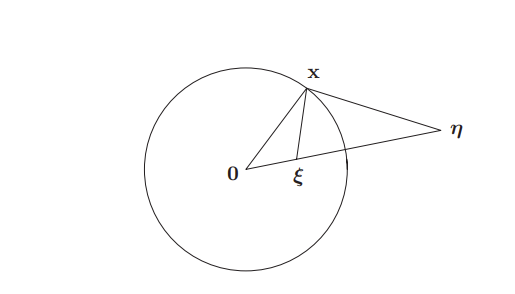
\includegraphics[width=0.5\textwidth]{MethodOfImages.png}
    \caption{Method of Images for a singular charge in a unit disk}
    \label{fig:MoI}
\end{figure}
Let us imagine an image charge at a point $\boldsymbol{\eta} \notin \bar{\Omega}$ as seen in Figure \ref{fig:MoI}. We shall write down the logarithmic potential due to the image charge $z(x,y)$ as follows
\begin{equation}
    z(x,y) =a \ln ||\vb{x} -\boldsymbol{\xi}|| + b \text{ for } \boldsymbol{\eta} \in\R^2 \backslash\bar{\Omega} \label{eq:2.39}
\end{equation}
Since $z(x,y)$ is harmonic everywhere except at $\boldsymbol{\eta}$, $z(x,y)$ is harmonic within $\Omega$ as well. For a Dirichlet boundary condition, we have the following two
\begin{equation}
\begin{split}
    \ln||\vb{x} - \boldsymbol{\xi}|| = a\ln ||\vb{x} &- \boldsymbol{\eta}|| + b \hspace{4pt} \forall\vb{x} \in \partial \Omega \\
    \text{or}
    \\
    ||\vb{x} - \boldsymbol{\xi}|| = \lambda||&\vb{x} - \boldsymbol{\eta}||^a \hspace{4pt} \forall\vb{x} \in \partial\Omega    
\end{split}
\end{equation}
where $\lambda = e^b$. We shall construct our triangle such that $\boldsymbol{\eta} = c\boldsymbol{\xi}$ and connects with $\vb{0}$. $\Delta \boldsymbol{0\xi}\vb{x}$ is similar with $\Delta \boldsymbol{0\eta}\vb{x}$. As a result, we have the following set of equalities
\begin{equation}
    \frac{\norm{\boldsymbol{\xi}}}{\norm{\vb{x}}} =
    \frac{\norm{\vb{x}}}{\norm{\boldsymbol{\eta}}} = \frac{\norm{\vb{x} - \boldsymbol{\xi}}}{\norm{\vb{x}-\boldsymbol{\eta}}} = \lambda \label{eq:2.41}
\end{equation}
with the last equality on being true if $a=1$. Let us choose 
\begin{equation}
    \norm{\boldsymbol{\eta}} = \frac{1}{\norm{\boldsymbol{\xi}}} \rightarrow \boldsymbol{\eta} = \frac{\boldsymbol{\xi}}{\norm{\boldsymbol{\xi}}^2} \label{eq:2.42}
\end{equation}
which then implies that $\vb{x}=1$ and lies on the boundary of the unit disk.
\begin{equation*}
    \norm{\vb{x}}^2 = \norm{\bs{\xi}}\,\norm{\bs{\eta}} = 1
\end{equation*}
As a result, we have $\lambda= \norm{\bs{\xi}}=\frac{1}{\norm{\bs{\eta}}}$ by \eqref{eq:2.41}. The relationship in \eqref{eq:2.42} is known as the inversion with respect to the unit circle of the point $\bs{\xi}$ to its image point $\bs{\eta}$. The following algebra will be useful
\begin{equation*}
    \norm{\bs{\xi}}
\,\norm{\vb{x}-\bs{\eta}} = \frac{\norm{\vb{x}-\bs{\eta}}}{\norm{\bs{\eta}}} = \frac{\norm{\vb{x}-\frac{\bs{\xi}}{\norm{\bs{\xi}}^2}}}{\frac{1}{\norm{\bs{\xi}}}}=\frac{\frac{1}{\norm{\bs{\xi}}^2}\norm{\vb{x}\norm{\bs{\xi}}^2-\bs{\xi}}}{\frac{1}{\norm{\bs{\xi}}}} = \frac{\norm{\,\norm{\bs{\xi}}^2\vb{x}-\bs{\xi}}}{\norm{\bs{\xi}}}
\end{equation*}
We now can see how this leads to the homogenous Dirichlet boundary conditions as
\begin{equation}
    \frac{1}{2\pi}\ln \norm{\vb{x} - \bs{\xi}} =\frac{1}{2\pi}\ln \left(  \norm{\bs{\xi}}
\,\norm{\vb{x}-\bs{\eta}}\right) = \frac{1}{2\pi}\ln \left( \frac{\norm{\,\norm{\bs{\xi}}^2\vb{x}-\bs{\xi}}}{\norm{\bs{\xi}}} \right)
\end{equation}
As such, we can add this with the free-space Green's Function to arrive at our solution
\begin{equation}
    \ggf = -\frac{1}{2\pi} \ln \norm{\vb{x} - \bs{\xi}} + \frac{1}{2\pi}\ln \frac{\norm{\,\norm{\bs{\xi}}^2\vb{x}-\bs{\xi}}}{\norm{\bs{\xi}}} = \frac{1}{2\pi} \ln \frac{\norm{\,\norm{\bs{\xi}}^2\vb{x}-\bs{\xi}}}{\norm{\bs{\xi}}\, \norm{\vb{x}-\bs{\xi}}}
\end{equation}
Changing to polar coordinates with 
\begin{equation*}
    \vb{x} = (r \cos \theta, r\sin\theta) \hspace{20pt} \bs{\xi} = (\rho \cos \phi, \rho \sin \phi)
\end{equation*}
and using the Law of Cosines for the triangle in Figure \ref{fig:MoI}, we can write the expression explicitly as 
\begin{equation}
    G(r,\theta; \rho,\phi)=\frac{1}{4\pi} \ln \frac{1+r^2\rho ^2-2r\rho \cos(\theta-\phi)}{r^2+\rho^2-2r\rho \cos(\theta - \phi)} \label{eq:2.45}
\end{equation}
Now we just need to evaluate the derivative of the Green's function at the border $\rho = 1$
\begin{equation}
    \pd{G}{\rho}(r,\theta;1,\phi) =-\frac{1}{2\pi}\frac{1-r^2}{1+r^2-2r\cos (\theta - \phi)} \label{eq:2.46}
\end{equation}

\begin{theorem}
    The solution to the inhomogeneous Dirichlet boundary value problem 
    \begin{equation*}
        -\lap u = f \text{ for } r=\norm{\vb{x}} < 1 \text{ and } u=h \text{ for } r=1
    \end{equation*}
    is, when expressed in polar coordinates
    \begin{equation}
    \begin{split}
        u(r,\theta) = &\frac{1}{4\pi}\int^\pi_{-\pi}\int^1_0 f(\rho,\phi)\ln \left( \frac{1+r^2 \rho^2-2r \rho \cos (\theta-\phi)}{r^2+\rho^2-2r\rho \cos(\theta-\phi)}\right) \rho d \rho  d\phi \\
        +&\frac{1}{2\pi}\int^\pi_{-\pi} h(\phi) \frac{1-r^2}{1+r^2-2r\cos (\theta - \phi)} d\phi
    \end{split}
    \end{equation}
\end{theorem}
\begin{proof}
    Apply Theorem 2.6 using Equations \eqref{eq:2.45} and \eqref{eq:2.46}.
\end{proof}
When $f\equiv0$, we get the Poisson integral formula which can find the value inside a domain given the values along the boundaries. It is analogous to the Cauchy Integral Formula from complex analysis. If the boundary data is $h(\theta) = \delta(\theta - \phi)$, we get the Poisson kernel 
\begin{equation}
    u(r,\theta) =\frac{1-r^2}{2\pi(1+r^2-2r\cos (\theta - \phi))}
\end{equation}

\newpage






\section{Evolution of Linear and Nonlinear Equations}



\textbf{The Fundamental Solution to the Heat Equation} \\
The Fourier series solution to the heat equation is sometimes not explicit enough for certain applications. As such, we desire a closed form fundamental solution to the heat equation. What we desire are the Green's Functions for the heat equation. We want to find how the heat diffuses from an initial, concentrated source of heat at a position $\xi$ along the bar. Let us denote the fundamental solution as 
\begin{equation}
    u(t,x) = F(t,x;\xi) \text{ with initial data } F(0,x;\xi) = \delta(x-\xi)
\end{equation}
and is a function for $t>0$ and $x$ and solves the \textit{heat equation} 
\begin{equation}
    \pd{F}{t} = \gamma \pdt{F}{x} \label{eq:heat}
\end{equation}
where $\gamma$ is the thermal diffusivity and represents how fast heat spreads within a material. The larger $\gamma$ is, the better the material conducts heat. Once again, we can represent the initial data as the linear superposition of delta functions weighted by the magnitude of the initial temperature distribution $f(x)$ at every point along the bar
\begin{equation*}
    u(0,x) = f(x) =\int^b_a \delta(x-\xi) f(\xi)d\xi
\end{equation*}
and represent the solution as the linear superposition of the fundamental response weighted by the magnitude at each point
\begin{equation*}
    u(t,x) = \int^b_aF(t,x;\xi)f(\xi)d\xi
\end{equation*}
Most boundary value problems do not have a closed form solution. However, one that does is the infinitely long and uniform bar.
\begin{equation}
    \pd{u}{t} = \pdt{u}{x} \text{ for } -\infty<x<\infty \text{ and } t>0 \label{eq:3.3}
\end{equation}
with an initial temperature distribution 
\begin{equation*}
    u(0,x) = f(x)
\end{equation*}
For the solution to uniquely exist, we require it to be square integrable for all $t>0$. This acts as the ``boundary conditions" as square integrability requires $|u(t,x)|$ to be vanishingly small at $x=\pm \infty$. To solve the initial value problem, let us take the Fourier Transform of \eqref{eq:3.3} and the initial conditions to get 
\begin{equation}
    \pd{\hat{u}}{t} =-k^2\hat{u} \text{ and } \hat{u}(0,k) =\hat{f}(k) = \frac{1}{\sqrt{2\pi}}\int^\infty_{-\infty} f(x)e^{-ikx}dx \label{eq:3.4}
\end{equation}
For clarity's sake, this document will use the Fourier Transform of a function $f(x)$ as
\begin{equation*}
    \mathscr{F}(f(x)) = \hat{f}(k) =\frac{1}{\sqrt{2\pi}}\int^\infty_{-\infty} f(x)e^{-ikx}dx
\end{equation*}
and the inverse Fourier Transform as 
\begin{equation*}
    \mathscr{F}^{-1}(\hat{f}(k)) = f(x)= \frac{1}{\sqrt{2\pi}} \int^\infty_{-\infty} \hat{f}(k)e^{ikx}dx
\end{equation*}
The solution to \eqref{eq:3.4} is trivially 
\begin{equation}
    \hat{u}(t,k) =e^{-k^2t}\hat{f}(k)
\end{equation}
By applying the inverse transform, we get that 
\begin{equation}
    u(t,x) =\frac{1}{\sqrt{2\pi}}\int^\infty_{-\infty}\hat{f}(k)e^{ikx-k^2t} dk \label{eq:3.6}
\end{equation}
Since we are finding the fundamental solution, our initial heat distribution is a delta function centered at $x=\xi$ so 
\begin{equation*}
    \mathscr{F}(\delta(x-\xi)) = \frac{e^{-ik\xi}}{\sqrt{2\pi}}
\end{equation*}
and plugging this into \eqref{eq:3.6} gets us that the fundamental solution is 
\begin{equation}
    F(t,x;\xi) =\frac{1}{2\pi}\int^\infty_{-\infty}e^{ik(x-\xi)-k^2t}dk = \frac{1}{2\sqrt{\pi t}}e^{\frac{-(x-\xi)^2}{4t}} \hspace{4pt} \forall t>0
\end{equation}
which one can figure out either through a table of Fourier Transforms or by completing the square of the exponential and performing a convenient substitution. 
The integral of the fundamental solution is a constant value which indicates the conservation of thermal energy.
\begin{equation*}
    \int^\infty_{-\infty} F(t,x;\xi) dx = 1
\end{equation*}
We can also see that as $t\rightarrow0^+$, then $F(t,x;\xi)$ becomes the delta function centered at $x=\xi$ (recall the sequence of functions interpretation of the Dirac delta). Some interesting things to note is that immediately after $t=0$, the temperature distribution turns into a series of ever-widening \textit{normal distributions} and is hence why the fundamental solution is often called a \textit{Gaussian filter}. It is also worth mentioning that the propagation of heat along the entire beam is instant which is clearly in violation of the laws of relativity. Otherwise, it is still an accurate model for heat propagation. Using the fundamental solution, we can construct the general solution to be 
\begin{equation}
    u(t,x) =\frac{1}{2\sqrt{\pi t}}\int^\infty_{-\infty} e^{-\frac{(x-\xi)^2}{4t}}f(\xi)d\xi
\end{equation}
This can also be thought of as a convolution between the fundamental solution to the heat equation centered at $\xi =0$ with the initial temperature distribution $f(x)$
\begin{equation}
    u(t,x) =F_0(t,x) *f(x) \text{ where } F_0(t,x)=F(t,x;0) = \frac{1}{2\sqrt{\pi t}}e^{-\frac{x^2}{4t}}
\end{equation}
and $*$ is the convolution operator 
\begin{equation*}
    f(t)*g(t) =\int_0^tf(\tau)g(t-\tau)d\tau
\end{equation*}
\textbf{The Forced Heat Equation} \\
Now we want to find the \textit{general fundamental solution} to the heat equation due to some forcing function $h(t,x)$. As such, let us apply a delta heat distribution at position $x=\xi$ and during time $t=\tau$. In other words, we are attempting to solve the equation
\begin{equation*}
    \pd{u}{t} = \pdt{u}{x} +\delta(t-\tau)\delta(x-\xi)
\end{equation*}
We will impose homogeneous initial conditions (there is no heat in the bar at $t=0$) and the solution will be the general fundamental solution to the heat equation.
\begin{equation*}
    u(t,x) = \gfsh
\end{equation*}
Due to the homogeneous initial conditions, it is useful to note that 
\begin{equation}
    \gfsh =0 \hspace{4pt} \forall t\leq \tau \label{eq:3.10}
\end{equation}
Once again, we can write the general forcing function as a superposition of delta functions 
\begin{equation}
h(t,x) =\int^\infty_0 \pull \int^b_a\delta (t-\tau)\delta(x-\xi)h(\tau,\xi) d\xi d\tau
\end{equation}
The general solution is 
\begin{equation*}
    u(t,x) = \int_0^\infty\pull \int^b_a \gfsh h(\tau, \xi)d\xi d\tau 
\end{equation*}
We can be a little bit more clever by splitting the $\tau$ integral into 
\begin{equation*}
    u(t,x) = \int^t_0(\ldots)d\tau +\int_t^\infty(\ldots)d\tau
\end{equation*}
In the second integral, we note that $t \leq \tau$ which means we can apply the condition in \eqref{eq:3.10} and therefore the second integral is 0 and we are left with 
\begin{equation}
    u(t,x) =\int^t_0\pull\, \int^b_a \gfsh h(\tau,\xi)d\xi d\tau \label{eq:3.12}
\end{equation}
For a non-homogeneous initial condition $f(x)$, we can express the solution as the superposition between the fundamental solution to the homogeneous heat equation and \eqref{eq:3.12} 
\begin{equation}
    u(t,x) = \int^b_a F(t,x;\xi)f(\xi) d\xi + \int^t_0\pull\, \int^b_a \gfsh h(\tau,\xi)d\xi d\tau 
\end{equation} 
We will now solve for the general fundamental solution for an infinitely long homogeneous bar. We shall once again take the Fourier transform of both sides to arrive at 
\begin{equation}
    \pd{\hat{u}}{t} +k^2\hat{u} = \frac{1}{\sqrt{2 \pi}}e^{-ik\xi} \delta (t-\tau)
\end{equation}
Since we are taking on homogeneous initial conditions, $\hat{u}(0,k) = 0$ as well. We then use an integrating factor of the form $e^{k^2t}$
\begin{equation*}
    \pd{}{t}\left( e^{k^2t}\hat{u}\right) = \frac{1}{\sqrt{2\pi}}e^{k^2t-ik\xi} \delta(t-\tau)
\end{equation*}
By then integration with respect from $0\rightarrow t$ and rearranging, we are left with 
\begin{equation}
    \hat{u}(t,k)=\frac{1}{\sqrt{2\pi}}e^{-k^2(t-\tau)+ik(x-\xi)}\sigma(t-\tau)
\end{equation}
Taking the inverse Fourier Transform yields
\begin{equation}
    u(t,x)=\gfsh =\frac{\sigma (t-\tau)}{2\sqrt{\pi (t-\tau)}}\exp\left[{\displaystyle{-\frac{(x-\xi)^2}{4(t-\tau)}}}\right] = \sigma(t-\tau)F(t-\tau,x;\xi) 
\end{equation}
Substituting this into \eqref{eq:3.12}, we obtain
\begin{equation}
    u(t,x)=\int^t_0 \pull\,\int_{-\infty}^\infty \frac{h (\tau,\xi)}{2\sqrt{\pi(t-\tau)}}\exp \left[ -\frac{(x-\xi)^2}{4(t-\tau)} \right]d\xi d\tau \label{eq:3.17}
\end{equation}
This is a demonstration of Duhamel's Principle which effectively states that when you have an inhomogeneity over time, we first obtain the impulse response. Then we can sum up all of the impulse responses over all time and space to find the response to the inhomogeneity. We can once again write \eqref{eq:3.17} as a convolution but this time in both space and time
\begin{equation}
    u(t,x) = h(t,x) * G(t,x;0,0)
\end{equation}
\textbf{The Black-Scholes Equation}\\
The most influential equation in quantitative finance is the Black-Scholes Equation
\begin{equation}
    \pd{u}{t} +\frac{\sigma^2}{2}x^2\pdt{u}{x}+rx\pd{u}{x} -ru= 0
\end{equation}
I genuinely have no idea what any of these terms. As such, I will just be copying Olver's explanation. The dependent variable $u(t,x)$ represents the monetary value of a single financial option, meaning a contract to either buy or sell and asset at a specified exercise price $p$ at a certain future time $t_\star$. The value $u(t,x)$ of the option will depend on the current time $t\leq t_\star$ and the current price $x\geq0$ of the underlying asset. As with many financial models, one assumes the absence of arbitrage, meaning that there is no way to make a riskless profit. The constant $\sigma>0$ represents the asset's volatility, while $r$ denotes the (assumed to be constant) interest rate for bank deposits, where investors could place their money with a guaranteed rate of return instead of buying the option. If we rearrange the Black-Scholes equation such that all the $x$ derivatives are one side we see that the Black-Scholes equation is a backwards diffusion process since the second spatial derivative is negative. 
\begin{equation}
    \pd{u}{t} = -\frac{\sigma^2}{2}x^2\pdt{u}{x}-rx\pd{u}{x} +ru 
\end{equation}
In contrast to the standard heat equation, the Black-Scholes equation is only well posed when run in reverse time. This gives rise to a \textit{final value problem} as opposed to an initial value problem. We want to determine the option value at the current time and asset value given the final condition
\begin{equation}
    u(t_\star,x) =f(x)
\end{equation}
For the \textit{European call option} where the option is to be bought at a price $p > 0$ at the specified time, the final condition is 
\begin{equation*}
    u(t_\star,x) = \max \{x-p,0\}
\end{equation*}
and for the \textit{put option} (where the option is to be sold), the final condition is 
\begin{equation*}
    u(t_\star,x) = \max \{p-x,0\}
\end{equation*}
The solution will be defined for all $t\leq t_\star$ and $x>0$ and subject to the boundary conditions
\begin{equation*}
    u(t,0) = 0 \text{ and } u(t,x) \approx x \text{ as } x\rightarrow \infty
\end{equation*}
The first step is to convert it into a forward diffusion process using the change of variables 
\begin{equation}
    \tau = \frac{1}{2} \sigma^2(t_\star -t) \hspace{20pt} v(\tau,x) = u\left(t_\star - \frac{2\tau}{\sigma^2},x \right)
\end{equation}
This has the effect of turning the final condition into an initial condition. Using the chain rule, the Black-Scholes equation turns into 
\begin{equation}
    \pd{v}{\tau} =x^2\pdt{v}{x} +\kappa x\pd{v}{x}-\kappa v \text{ where } \kappa =\frac{2r}{\sigma^2}
\end{equation}
The next thing to do is remove the explicit dependence on $x$ for the right hand side. This is done by recognizing that the right hand side takes the form of an Euler differential equation. We therefore have
\begin{equation}
    w(\tau,y) = v(\tau,e^y)=v(\tau,x)
\end{equation}
By computing the derivatives using the chain rule we get 
\begin{equation}
    \pd{w}{\tau} = \pdt{w}{y}+(\kappa -1)\pd{w}{y} -\kappa w \label{eq:3.25}
\end{equation}
We can finally arrive at the heat equation by writing $w(\tau,y)$ as 
\begin{equation}
    w(\tau,y) = e^{\alpha \tau+\beta y}z(\tau,y)    
\end{equation}
Substituting this into \eqref{eq:3.25} yields
\begin{equation}
    \pd{z}{\tau} +\alpha z= \pdt{z}{y} +\beta^2 z+(\kappa-1)\left( \pd{z}{y}  +\beta z\right) - \kappa z
\end{equation}
We can eliminate the $\pd{z}{y}$ and $z$ terms by setting 
\begin{equation*}
    \alpha = -\frac{1}{4}(\kappa +1)^2 \hspace{20pt}\beta = -\frac{1}{2}(\kappa-1)
\end{equation*}
and therefore the function 
\begin{equation}
    z(\tau,y) =e^{\frac{(\kappa+1)^2\tau}{4}+\frac{(\kappa-1)y}{2}}w(\tau,y)
\end{equation}
satisfies the heat equation
\begin{equation}
    \pd{z}{\tau} = \pdt{z}{y}
\end{equation}
\begin{proposition}
    If $z(\tau,y)$ is a solution to the initial value problem 
    \begin{equation*}
        \pd{z}{\tau} = \pdt{z}{y} \hspace{20pt} z(0,y)=h(y) = e^{\frac{(\kappa-1)y}{2}}f(e^y)
    \end{equation*}
    for $\tau>0$, $-\infty < y <\infty$, then 
    \begin{equation*}
        u(t,x)=x^{-\frac{\kappa-1}{2}}e^{-\frac{1}{8}(\kappa+1)^2\sigma^2(t_\star-t)} z(\frac{1}{2}\sigma^2(t_\star-t),\ln x)
    \end{equation*}
    solves the final value problem for the European call option for $t\leq t_\star$ and $0<x<\infty$.
\end{proposition}
\begin{proof}
    Ask a toddler on the street.
\end{proof}
Through the analysis above, we know we can write the solution to the heat equation as the convolution between the initial data and the fundamental solution 
\begin{equation}
    z(\tau,y) = \frac{1}{\sqrt{2\pi \tau}}\int^\infty_{-\infty} e^{-\frac{(y-\eta)^2}{4\tau}+\frac{1}{2}(\kappa -1)\eta}f(e^\eta)d\eta \label{eq:3.30}
\end{equation} 
We can then combine \eqref{eq:3.30} with the solution for $u(t,x)$ in Proposition 3.1. Specifically for the European call option we arrive at the integral
\begin{equation}
    z(\tau,y)=\frac{1}{2\sqrt{\pi}}\int_{\log p}^{\infty} e^{-(y-\tau)^2/(4\tau)+(\tau-1)n/2}(e^{n}-p)\,d\eta
\end{equation}
By completing the square, we can evaluate the integral to be 
\begin{equation}
\begin{split}
    z(\tau, y) = \frac{1}{2}\left[ e^{(\kappa+1)^2 \tau/4 + (\kappa+1) y/2} \operatorname{erfc}\left( \frac{\log p - (\kappa + 1)\tau - y}{2 \sqrt{\tau}} \right) \right. \\ \left. - p e^{(\kappa-1)^2 \tau/4 + (\kappa-1) y/2} \operatorname{erfc}\left( \frac{\log p - (\kappa - 1)\tau - y}{2 \sqrt{\tau}} \right) \right]
\end{split}
\end{equation}
erfc is the complementary error function which is defined to be 
\begin{equation*}
    \operatorname{erfc} x = 1-\operatorname{erf}x=1-\frac{2}{\sqrt{\pi}}\int^x_0 e^{-t^2}dt = \frac{2}{\sqrt{\pi}} \int^\infty_xe^{-t^2}dt
\end{equation*}
As such, the solution to the Black-Scholes equation for the European call option is 
\begin{equation*}
\begin{split}
    u(t,x) = \frac{1}{2}\left[ x\,\operatorname{erfc}\left(-\frac{\left(r + \tfrac{1}{2}\sigma^{2}\right)(t_\star - t) + \ln\frac{x}{p}}{\sqrt{2\,\sigma(t_\star - t)}}\right)  
    -\; p\, e^{-r(t_\star-t)}\operatorname{erfc}\left(-\frac{\left(r - \tfrac{1}{2}\sigma^{2}\right)(t_{\star} - t) + \ln\frac{x}{p}}{\sqrt{2\,\sigma(t_{\star} - t)}}\right)\right]
\end{split}
\end{equation*}
\textbf{Symmetries and Similarities} \\
A \textit{symmetry} of an equation is a transformation that takes one solution to another solution. By knowing a symmetry of an equation, one can generate a second, third, or even more solution to the equation. The general study of the finding the symmetries of a differential equations falls under Lie Theory which is named after Norwegian mathematician Sophus Lie. Lie attempted to analyze the symmetries of the solutions to differential equations in the same way Galois Theory analyzed the roots of polynomials (and is the reason why there exists no quintic formula). It is blend of both group theory and differential geometry.\\\\ We shall use the heat equation to show off these symmetries. The first type of symmetry is a translation.
\begin{equation}
    t \mapsto t+a \hspace{20pt} x\mapsto x+b
\end{equation}
This type of transformation leads to 
\begin{equation*}
    \hat{t} =t+a, \ \hat{x}=x+b \rightarrow U(\hat{t},\hat{x}) =u(t,x) =u(\hat{t}-a,\hat{x}-b)
\end{equation*}
and so thus dropping the hats leads to the translated function to be 
\begin{equation}
    U(t,x) = u(t-a,x-b) \label{eq:3.34}
\end{equation}
Since the partial derivatives remain the same (as the constant goes to zero), $U(t,x)$ solves $U_t=\gamma U_{xx}$ when $u(t,x)$ solves $u_t=\gamma u_{xx}$. A translation symmetry indicates that we are working on a homogeneous medium since the solution doesn't depend on the reference point or choice of coordinates. Translation symmetries also produce an infinite family of solutions. One word of warning, translation symmetries do not respect initial or boundary conditions. As such, one must translate these conditions accordingly. For example, if a solution is defined for some time $t\geq 0$ and on a domain $0\leq x\leq l$, the appropriate initial and boundary conditions for the translated symmetry are $t\geq a$ and $b\leq x \leq x+b$. \\\\
Another important class of symmetries are \textit{scaling invariances}. This essentially takes a solution $u(t,x)$ and constructs another solution 
\begin{equation}
    U(t,x) = cu(t,x)+k
\end{equation}
for some arbitrary constants $c$ and $k$. This is effectively a change in the scale we are using (Celsius or Fahrenheit or some other wacko scale like Rankine). A more interesting scaling symmetry is by scaling the variables themselves
\begin{equation}
    t \mapsto \alpha t \hspace{20pt} x\mapsto \beta x
\end{equation}
Using a similar procedure that we used in \eqref{eq:3.34}, we arrive at the scaled solution to be 
\begin{equation}
    U(t,x) = u(\alpha^{-1}t, \beta^{-1}x)
\end{equation}
The partial derivatives are now scaled by these factors too. 
\begin{equation*}
    \pd{U}{t} = \frac{1}{\alpha} \pd{u}{t} \hspace{20pt} \pdt{U}{x} = \frac{1}{\beta^2}\pdt{u}{x}
\end{equation*}
Therefore, if $u(t,x)$ solves the equation $u_t = \gamma u_{xx}$, $U(t,x)$ solves the equation 
\begin{equation}
    \pd{U}{t} = \frac{1}{\alpha} \pd{u}{t} = \frac{\gamma}{\alpha}\pdt{u}{x} = \frac{\beta^2 \gamma}{\alpha}\pdt{U}{x}
\end{equation}
We then rewrite $\frac{\beta^2 \gamma}{\alpha} =\Gamma$ so we arrive at 
\begin{equation*}
    \pd{U}{t} = \Gamma \pdt{U}{x}
\end{equation*}
Physically, this just means that whenever we scale space and time, we just end up rescaling the diffusion coefficient. If we conveniently choose $\alpha =\gamma$ and $\beta =1$, the rescaled diffusivity is $\Gamma =1$. This leads to an useful observation. If $U(t,x)$ is a solution to the heat equation with unit diffusivity ($\Gamma =1$), then 
\begin{equation*}
    u(t,x) = U(\gamma t,x)
\end{equation*}
also solves the heat equation for $\gamma > 0$. By changing $\gamma$, we are effectively changing the time it takes for the object to heat/cool. An object with $\gamma=2$ will cool down twice as fast as the same object (subject to the same conditions) but with $\gamma =1$. If we use the transformation 
\begin{equation*}
    t\mapsto \beta^2t \hspace{20pt} x\mapsto \beta x
\end{equation*}
we get that the diffusion coefficient stays the same ($\Gamma =\gamma$). Combining this with a linear rescaling, we see that if $u(t,x)$ solves the heat equation $u_t = \gamma u_{xx}$, then 
\begin{equation}
    U(t,x) = cu(\beta^{-2}t, \beta^{-1}x)
\end{equation}
solves the heat equation for the \textit{same} diffusion coefficient. This is therefore a scaling invariance since it solves the \textit{same} differential equation with no rescaling. Once again, we must be vary of any initial and boundary conditions and scale them appropriately. For an object that is twice the length of another object made of the same material, we construct the scaled solution $U(t,x)$ with $\beta = 2$ and $\alpha =4$ and hence $U(t,x) = cu(\frac{1}{4}t, \frac{1}{2}x)$ and we come to the conclusion that an object twice as long will take four times longer to cool. \\ \\
\textbf{Similarity Solutions}\\
A similarity solution is one that remains invariant under any scaling symmetries. Suppose our PDE admits the scaling symmetries
\begin{equation}
    t\mapsto\beta^at \hspace{20pt} x\mapsto\beta^bx \hspace{20pt} u\mapsto\beta^cu \hspace{20pt}\beta\neq 0
\end{equation}
where $a,b,c$ are constants and $a,b \neq0$. As a result, the rescaled solution would be 
\begin{equation}
    U(t,x) = \beta^cu(\beta^{-a}t,\beta^{-b}x) \label{eq:3.41}
\end{equation}
$u(t,x)$ is a similarity solution if the left hand side of \eqref{eq:3.41} is $U(t,x) = u(t,x)$. For the following example, let us assume $a\neq 0$. Since the left hand side is completely independent of $\beta$ and ``anchored" by the specific $t$ and $x$, our scaling symmetry should work for all $\beta > 0$. Let us choose a convenient $\beta = t^{1/a}$ such that it eliminates one of our variables. We now have 
\begin{equation}
    u(t,x) =t^{c/a}v(\xi) \hspace{20pt} \xi = xt^{-b/a} \hspace{20pt} v(\xi) = u(1,\xi) \label{eq:3.42}
\end{equation}
$\xi$ is called the similarity variable. The next steps are to find the partial derivatives of $u(t,x)$ in terms of ordinary derivatives of $v(\xi)$ and then substituting it back into the scale invariant PDE. This then reduces the problem to an ODE. Let us take a look at an example using the nonlinear transport equation. Taking the chain rule and substituting it into \eqref{eq:1.11} gets us 
\begin{equation}
    \beta^{c-a}u_t+\beta^{2c-b}u_{x} = 0
\end{equation}
We require all the $\beta$s to be raised to the same power (in order to factor them out and recover the original equation) and so thus $2c-b=c-a \rightarrow c=b-a$. Let us choose $a=1$ to make things easy and as a result, we have $c=b-1$. We now employ the ansatz from \eqref{eq:3.42} to obtain 
\begin{equation}
    u(t,x) =t^{b-1}v(\xi) \hspace{20pt} \xi =xt^{-b} \label{eq:3.44}
\end{equation}
Differentiating $u(t,x)$ and doing some factoring leaves us with 
\begin{equation}
    u_t =t^{b-2}[-b\xi v'(\xi)+(b-1)v(\xi)] \hspace{20pt} u_x=t^{-1}v'(\xi)
\end{equation}
and substituting this into the nonlinear transport equation gets us the ordinary differential equation
\begin{equation}
    (v-b)\od{v}{\xi} +(b-1)v=0
\end{equation}
If $b=1$, either $v=b\xi$ or $v$ is constant. Otherwise, we solve the differential equation but for $\xi$ as a function of $v$. 
\begin{equation*}
    (b-1)v\od{v}{\xi} -b\xi=-v
\end{equation*}
This equation can be solved by an integrating factor and thus we get 
\begin{equation*}
    \xi=v+kv^\frac{b}{b-1}
\end{equation*}
where $k$ is an integration constant. By making use of the identities from \eqref{eq:3.44}, $v=u/t^{b-1}$ and $\xi =x/t^b$, we arrive at 
\begin{equation*}
    x=ku^\frac{b}{b-1}+tu
\end{equation*}
\textbf{The Maximum Principle}\\
Thermodynamics tells us that the overall heat content of a certain body must continually decrease. The Maximum Principle is the mathematical formulation and states that in the absence of external heat sources, the temperature inside an object cannot exceed the initial boundary values.
\begin{theorem}[The Weak Maximum Principle]
    Let $\gamma >0$. Suppose $u(t,x)$ is a solution to the forced heat equation 
    \begin{equation*}
        \pd{u}{t} = \gamma \pdt{u}{x} + F(t,x)
    \end{equation*}
    on the rectangular domain 
    \begin{equation*}
        R=\{a\leq x \leq b, 0 \leq t \leq c \}
    \end{equation*}
    Assuming that the forcing term is nowhere positive, $F(t,x) \leq 0$, then the maximum of $u(t,x)$ on the closed rectangle $\bar{R}$ is attained at $t=0, x=a,$ or $x=b$.
\end{theorem}
\begin{proof}
    Let us first prove the result under the stronger assumption that $F(t,x) = \pd{u}{t} -\gamma \pdt{u}{x} <0$ which implies $\pd{u}{t} < \gamma \pdt{u}{x}$ everywhere in $R$. Suppose there exists a point $(t^\star, x^\star) \in R$ such that $u(t,x)$ is at a local maximum. By definition, its gradient must be 0.
    \begin{equation*}
        \nabla u(t^\star, x^\star ) = \vb{0} \rightarrow u_t(t^\star,x^\star) = u_{x}(t^\star, x^\star) = 0
    \end{equation*}
    Now let us assume a scalar function $h(x) = (t_\star, x)$. $h(x)$ has a maximum at $x=x^\star$ which means by the second derivative test,
    \begin{equation*}
        h''(x^\star) = u_{xx}(t^\star, x^\star) \leq 0
    \end{equation*}
    This is impossible since we showed earlier that $u_t < u_{xx}$ but $u_t = 0$ and $u_{xx} \leq 0$. As such, our initial assumption that there exists a maximum within $R$ is false. Now we need to exclude the possibility of the maximum occurring at the right edge of the rectangle at a point $(t^\star,x^\star) = (c,x^\star)$ where $a<x^\star < b$. If this is the case, then $g(t) =u(t,x^\star)$ is nondecreasing with respect to time at $t=c$ which implies $g'(t) = u_t(t,x^\star) \geq 0$ which is once again with the conditions we established earlier. \\\\
    To generalize our results to the $F(t,x) \leq 0$, we start with a solution to the forced heat equation $u(t,x)$ and add a little perturbation.
    \begin{equation*}
        v(t,x) = u(t,x) + \varepsilon x^2 \text{ where } \varepsilon>0
    \end{equation*}
    By the chain rule, we get the following 
    \begin{equation*}
        \pd{v}{t} = \pd{u}{t} =\gamma \pdt{u}{x}+F(t,x) = \gamma \pdt{v}{x} -2\gamma \varepsilon+F(t,x) = \gamma \pdt{v}{x} +\tilde{F}(t,x)
    \end{equation*}
    Since $F(t,x) \leq 0$ and $\varepsilon>0$, we know that 
    \begin{equation*}
        \tilde{F}(t,x) = F(t,x) -2\gamma\varepsilon <0
    \end{equation*}
    and we can use what we proved previously to state that $v(t,x)$ cannot attain a a maximum anywhere in $R$ or on the right edge of $R$. Now to rigorously show that this applies to $u(t,x)$, let us denote the maximum value of $u(t,x)$ on any of the three sides as $M$. By our previous logic and mimicking the form of $v(t,x)$, we get
    \begin{equation*}
    u(t,x) \leq v(t,x) \leq M+\varepsilon \max \{a^2,b^2 \}.
    \end{equation*}
    Now let $\varepsilon\rightarrow 0^+$ and we have $u(t,x) \leq M$ everywhere in $R$.
    
\end{proof}
This is known as the \textit{Weak Maximum Principle}. The \textit{Strong Maximum Principle} states that given a non-constant solution $u(t,x)$, any non-initial, non-bonudary point $(t,x) \in \hat{R} = \{a<x<b, 0<t\leq c\}$ is strictly less than its maximum initial and boundary values. In math terms, $u(t,x)<M \ \forall(t,x)\in \hat{R}$. Since the Maximum Principle is used to establish Corollary \ref{coro:mM}, the inequalities become strict in there as well. 
\begin{corollary}
    Supposed $u(t,x)$ solves the heat equation $u_t = \gamma u_{xx}$ with $\gamma > 0$ for $a,x<b$ and $0<t<c$. Set 
    \begin{equation*}
        B=\{(0,x) \ | \ a\leq x \leq b\} \cup \{(t,a)\ | \ 0\leq t \leq c\} \cup \{(t,b)\ | \ 0 \leq t \leq c\}
    \end{equation*}
    and let 
    \begin{equation*}
        M = \max \{u(t,x) \ | \ (t,x) \in B\} \hspace{20pt} m=\min \{u(t,x) \ | \ (t,x) \in B \}
    \end{equation*}
    be respectively the maximum and minimum values for the initial and boundary temperatures. Then $m \leq u(t,x) \leq M$ for all $a \leq x \leq b, 0 \leq t \leq c$.\label{coro:mM}
\end{corollary}
\begin{proof}
        The upper bound $u(t,x) \leq M$ follows immediately from the Maximum principle. To establish the lower bound, let us define a new function $\tilde{u}(t,x) = -u(t,x)$ that also solves the heat equation. This satisfies $\tilde{u}(t,x) \leq -m$ on $B$ by the Maximum Principle (in essence what we're doing is flipping the sign such that the minimum now becomes the maximum). This implies that $u(t,x) = -\tilde{u}(t,x) \geq m$.
    \end{proof}
\begin{theorem}[Uniqueness]
    There is at most, one solution to the Dirichlet initial-boundary value problem for the forced heat equation.
\end{theorem}
\begin{proof}
    Suppose $u$ and $\tilde{u}$ are any two solutions to the forced heat equation with the same initial and boundary value conditions. Their difference $v=u-\tilde{u}$ then solves the homogeneous initial-boundary value problem for the unforced heat equation (since the forcing terms cancel out). By the Maximum Principle and Corollary \ref{coro:mM}, we get the maximum and minimum must appear on the boundaries and therefore $m=0\leq v(t,x) \leq M=0$ everywhere which implies $u\equiv \tilde{u}$ and therefore $u$ is unique.
\end{proof}
\textbf{Nonlinear Diffusion} \\
The nonlinear transport equation \eqref{eq:1.11} is known as the inviscid Burgers' Equation due to the lack of a viscous term. By including a viscous term, we arrive at the viscous Burgers' Equation.
\begin{equation}
    \pd{u}{t}+u\pd{u}{x} = \gamma \pdt{u}{x}
\end{equation}
For solutions with small magnitudes of $|u(t,x)|$, the solutions tend to behave similar to the heat equation since the first spatial derivative term is weighted less. For large $|u(t,x)|$, the first spatial term tends to dominate the temporal derivative. Generally, we have the conditions to be 
\begin{equation*}
    u(0,x) = f(x) \hspace{20pt} -\infty<x<\infty
\end{equation*}
The simplest solutions are traveling wave solutions, where we once again travel along the characteristic 
\begin{equation*}
    u(t,x) = v(\xi) = v(x-ct)
\end{equation*}
By employing the chain rule, we can turn Burgers' Equation into the following nonlinear ordinary differential equation
\begin{equation}
    -cv'+vv'= \gamma v''
\end{equation}
Integrating both sides we get 
\begin{equation*}
    \gamma v' = k - cv+\tfrac{1}{2}v^2
\end{equation*}
We can factor the right hand side to become 
\begin{equation}
    2\gamma \od{v}{\xi} = (v-a)(v-b) \text{ where } c=\tfrac{1}{2}(a+b) \hspace{20pt} k=\tfrac{1}{2}ab
\end{equation}
In order to prevent the solution from blowing up to infinity, we need $v$ to be between the fixed points $a,b$. Integrating by separation of variables gets 
\begin{equation}
    \int\frac{2\gamma dv}{(v-a)(v-b)} = \frac{2\gamma}{b-a}\ln \left( \frac{b-v}{v-a} \right) = \xi -\delta
\end{equation}
where $\delta$ is a constant of integration. Solving for $v$ we get 
\begin{equation*}
    v(\xi) =\frac{ae^{\frac{1}{2\gamma}(b-a)(\xi-\delta)}+b}{e^{\frac{1}{2\gamma}(b-a)(\xi -\delta)}+1}
\end{equation*}
Substituting in for the characteristic variable gets 
\begin{equation}
    u(t,x) =v(\xi) =\frac{ae^{\frac{1}{2\gamma}(b-a)(x-ct-\delta)}+b}{e^{\frac{1}{2\gamma}(b-a)(x-ct -\delta)}+1}
\end{equation}
\textbf{Hopf-Cole Transformation} \\
Burgers' Equation can be linearized to become the heat equation and therefore be solved explicitly. Not all nonlinear differential equations can be linearized but when it is possible, it makes life a lot easier. Let us first start with the heat equation 
\begin{equation*}
    v_t = \gamma v_{xx}
\end{equation*}
We shall employ the exponential change of variables 
\begin{equation*}
    v(t,x) = e^{\alpha \varphi(t,x)} \rightarrow \varphi(t,x) = \frac{1}{\alpha}\ln (v(t,x))
\end{equation*}
where $\alpha \neq 0$ and $v(t,x)$ is strictly positive. We can achieve this by just having the initial data to be strictly positive as by the Maximum Principle and Corollary \ref{coro:mM}, we will have $v(t,x) > 0$ if $v(0,x)$. Differentiating and applying the chain rule we get 
\begin{equation*}
    v_t = \alpha\varphi_te^{\alpha \varphi} \hspace{20pt} v_x = \alpha v_x e^{\alpha \varphi} \hspace{20pt} v_{xx} = (\alpha \varphi_{xx}+\alpha^2\varphi_x^2)e^{\alpha \varphi} 
\end{equation*}
Canceling out the exponential term leaves us with what is known as the \textit{potential Burgers' Equation}. 
\begin{equation}
    \varphi_t= \gamma\varphi_{xx}+\gamma\alpha \varphi_x^2 \label{eq:pbe}
\end{equation}
If we now differentiate both sides with respect to $x$, we get
\begin{equation}
    \varphi_{xt} = \gamma \varphi_{xxx}+2\gamma \alpha \varphi_{x} \varphi_{xx} \label{eq:3.53}
\end{equation}
If we let $\varphi_x=u$ and $\alpha =-\frac{1}{2\gamma}$, we arrive at Burgers' equation.
\begin{equation*}
    u_t = \gamma u_{xx} + 2\gamma \alpha uu_{x}
\end{equation*}
The Hopf-Cole transformation is now complete.
\begin{theorem}
    If $v(t,x) >0$ is any positive solution to the linear heat equation $v_t=\gamma v_{xx}$, then 
    \begin{equation}
        u(t,x) =\pd{}{x} [-2\gamma \ln(v(t,x))] =  -2\gamma \frac{v_x}{v}
    \end{equation}
    solves Burgers' equation $u_t +uu_x = \gamma u_{xx}$.
\end{theorem}
\begin{proof}
    Let us first choose a potential function $\tilde{\varphi} (t,x) $ such that it solves the equation 
    \begin{equation*}
        \od{\tilde{\varphi}}{x} = u \rightarrow \tilde{\varphi}(t,x) = \int^x_0 u(t,y)dy
    \end{equation*}
    If $u(t,x)$ satisfies Burgers' Equation, then $\tilde{\varphi}(t,x)$ satisfies \eqref{eq:3.53}. If we integrate both sides of \eqref{eq:3.53} with respect to $x$, we end up having $g(t)$ as a constant of integration.
    \begin{equation*}
        \tilde{\varphi}_t = \gamma \tilde{\varphi}_{xx} +\gamma \alpha \tilde{\varphi}_x^2 + g(t)
    \end{equation*}
    We have this constant of integration because we chose the ``wrong" potential function (unless $g(t) \equiv 0$). The correct potential function is $\varphi(t,x) = \tilde{\varphi}(t,x) -G(t)$ where $G'(t) = g(t)$. As such, we arrive at potential Burgers' Equation
    \begin{equation*}
        \varphi_t = \tilde{\varphi}_t - g(t) = \gamma \tilde{\varphi}_{xx} +\gamma \alpha \tilde{\varphi}_x^2 + g(t) - g(t) =\gamma \varphi_{xx} +\gamma \alpha \varphi_x^2
    \end{equation*}
    By then reverting the exponential change of variables we get that $v(t,x) = e^{\alpha \varphi(t,x)}=e^{-\varphi (t,x)/2\gamma}$. Reversing this, we can easily prove the theorem. We can thus conclude that every solution to Burgers' Equation comes from a positive solution to the heat equation.
\end{proof}
\textbf{Linear Dispersion}\\
The simplest nontrivial third-order partial differential equation is 
\begin{equation}
    u_t + u_{xxx} = 0 \label{eq:3.55}
\end{equation}
which model dispersive waves that propagate unidirectionally. Since there is only a first derivative in time, we only need one initial condition to expect unique solutions.
\begin{equation*}
    u(0,x) = f(x) \hspace{20pt}-\infty < x <\infty
\end{equation*}
Assuming that $u(t,x)$ is square integrable (where $u(t,x)$ represents the wave height), we take the Fourier Transform to arrive at 
\begin{equation*}
    \pd{\hat{u}}{t} +(ik)^3\hat{u} = \pd{\hat{u}}{t} -ik^3\hat{u} = 0
\end{equation*}
The solution to the initial value problem here is trivially 
\begin{equation*}
    \hat{u}(t,x) = \hat{f}(k) e^{ik^3t}
\end{equation*}
By inverting, we get that the solution \eqref{eq:3.55} is 
\begin{equation}
    u(t,x) = \frac{1}{\sqrt{2\pi}} \int ^\infty_{-\infty} \hat{f}(k)e^{i(kx+k^3t)}dk
\end{equation}
Let us walk through an example. Let us find the fundamental solution to the dispersive wave equation. As is standard, the initial data is a delta function $u(0,x) = \delta (x)$. Since $\hat{\delta}(x) = \frac{1}{\sqrt{2\pi}}$ and the imaginary part of the exponential is odd, we have 
\begin{equation}
    u(t,x) = \frac{1}{2\pi}\int^\infty_{-\infty} e^{i(kx+k^3t)}dk = \frac{1}{\pi}\int^\infty_0 \cos(kx+k^3t)dk \label{eq:3.57}
\end{equation}
Although it does not seem like it, the above integral does converge. The cubic $k^3$ term induces rapid oscillations that cancel out and therefore lead to convergence. We can find the integral by a non-trivial integration by parts 
\begin{equation}
\begin{split}
    \int^l_0 \cos(kx+k^3t)dk =& \int^l_0\frac{1}{x+3k^2t}\od{}{k} \sin(kx+k^3t)dk\\
    =&\frac{\sin(kx+k^3t)}{x+3k^2t} \bigg|^l_0 -\int^l_0\od{}{k} \left( \frac{1}{x+3k^2t}\right)\sin(kx+k^3t)dk \\
    =&\frac{\sin(lx+l^3t)}{x+3l^2t} -\int^l_0 \frac{6kt\sin(kx+k^3t)}{(x+3k^2t)^2}dk
\end{split}
\end{equation}
Assuming $t\neq 0$, we can see that the first term goes to 0 as $l\rightarrow \infty$ and the second term converges absolutely. While the integral in \eqref{eq:3.57} cannot be written in terms of elementary functions, it does take the form of the Airy Function which is of the form
\begin{equation*}
    \operatorname{Ai} (z) = \frac{1}{\pi}\int^\infty_0 \cos(sz+\tfrac{1}{3}s^3)ds
\end{equation*}
By undergoing the change of variables $s=k\sqrt[3]{3t}$ and $z=\frac{x}{\sqrt[3]{3t}}$, we can see that the \eqref{eq:3.57} can be written as 
\begin{equation*}
    u(t,x) = \frac{1}{\sqrt[3]{3t}} \operatorname{Ai}\left( \frac{x}{\sqrt[3]{3t}} \right)
\end{equation*}
We note that the equation is translationally invariant (to verify this, apply a shift in $x$ and $t$ and apply the chain rule and see if it satisfies the original equation) and as such, the fundamental solution to the linear dispersive equation \eqref{eq:3.55} due to an impulse at $x=\xi$ can be written as 
\begin{equation*}
    F(t,x;\xi)=\frac{1}{\sqrt[3]{3t}} \operatorname{Ai}\left( \frac{x-\xi}{\sqrt[3]{3t}} \right)
\end{equation*}
and accordingly, the general solution is 
\begin{equation}
    u(t,x) =\frac{1}{\sqrt[3]{3t}} \int^\infty_{-\infty} f(\xi)\operatorname{Ai}\left( \frac{x-\xi}{\sqrt[3]{3t}} \right) d\xi
\end{equation}
\textbf{Dispersion Relations}\\
To better understand why the third derivatives lead to dispersion, let us take a look at the dispersion relation. We want to start with a purely oscillatory wave. The reason for this is tied to the fact that for a constant coefficient differential operator (for example, $L = \partial_t+\partial_{xxx}$ for \eqref{eq:3.55}), the purely oscillatory wave of a complex exponential like $e^{i(kx-\omega t)}$, is an eigenfunction of the linear differential operator. Since we care about solutions that conserve a finite amount of energy, we are worried about the $L^2$ function space. Although our purely oscillatory function is not in the $L^2$ function space (one can verify this by taking the norm 
\begin{equation*}
    \int^\infty_{-\infty}|e^{ikx}|^2dx = \int^\infty_{-\infty}(e^{ikx})(e^{-ikx})dx = \int^\infty_{-\infty}1dx = \infty
\end{equation*}
by multiplying $e^{ikx}$ by its complex conjugate), the linear superposition due to a continuous sum leads to a function within $L^2$ (since we care about localized wave packets, for $x$ close to 0, a lot of waves add constructively and therefore result in a nonzero wave packet. However, for large $x$, slightly different values of $k$ lead to cancellation due to the rapid oscillations). As such, by understanding the dispersion relation using our purely oscillatory function, we can understand the dispersion relation for $L^2$ solutions. So we start with our ansatz
\begin{equation*}
    u(t,x) = e^{i(kx-\omega t)}
\end{equation*}
Differentiating, we get 
\begin{equation*}
    u_t = -i\omega u \hspace{20pt} u_{xxx} = -ik^3u
\end{equation*}
Substituting this back into \eqref{eq:3.55} and cancelling out $u$, we get the dispersion relation
\begin{equation}
    \omega = -k^3
\end{equation}
Substituting this into our exponential ansatz we get 
\begin{equation}
    u(t,x) = e^{i(kx+k^3t)} \label{eq:3.61}
\end{equation}
This should be familiar it is the Fourier Transform formula centered at $\xi=0$ we derived in \eqref{eq:3.57}. We can now see that the Fourier Transform formula is a linear superposition of all of these complex exponentials, the same justification we used to create our exponential ansatz. We can factor out a $k$ from the exponent which leads to 
\begin{equation}
    e^{ik(x-c_pt)} \hspace{20pt} c_p =\frac{\omega}{k}
\end{equation}
We can now see that the exponent is in the form of a traveling wave with \textit{phase velocity} $c_p$. For the linear transport equation, we get a dispersion relation of $\omega = ck$ so therefore get a phase velocity of $c_p = \frac{ck}{k} = c$ and all different frequency waves move at the same speed $c$. For the classical wave equation \eqref{eq:wave}, the dispersion relation $\omega ^2 = c^2k^2 \rightarrow \omega=\pm ck$ and we essentially arrive at the same dispersion relationship as for the linear transport equation; however, the one difference is that the plus-minus enables the existence of bidirectional waves. For \eqref{eq:3.57}, our dispersion relationship is $\omega = -k^3$ and so the phase velocity is $c_P = -k^2$. What this means is that for a larger \textit{wave number} $k=\frac{2\pi}{\lambda}$ (where $\lambda$ is the wavelength and $k$ represents the \textit{spatial frequency}), the faster the wave with that frequency moves to the left. \\\\
The dispersion relation only governs how individual frequency waves evolve, and not the bulk of the wave moves. To do follow the wave packet, let us perform the change of variables $x=ct+\xi$ which leads to \eqref{eq:3.61} to become 
\begin{equation}
    u(t,ct +\xi) =\int^\infty_{-\infty} e^{i(ck-\omega)t}e^{ik\xi}g(k) dk
\end{equation}
For a fixed value of $\xi$, we have the integral 
\begin{equation}
    H(t) = \int^\infty_{-\infty} e^{i\varphi (k)t}h(k)dk
\end{equation}
where $\varphi(k) =ck-\omega(k)$ and $h(k) =e^{ik\xi}g(k)$. We want to know how the integral behaves as $t\rightarrow \infty$. If $\varphi(k) =k$, we just have a Fourier integral and $H(t)\rightarrow0$ for reasonable $h(k)$. This is once again due to the rapid oscillation for large $t$ and so therefore the integral goes to 0. Something similar happens when $\varphi(k)$ has no fixed points as one can perform a change of variables that leads to $\tilde{k} =\varphi(k)$ and recover the Fourier integral. According to Stokes and Kelvin, the only parts of the integral that survive the cancellation are when $\varphi'(k) =0$. Evaluating a highly oscillatory integral like this is known as the \textit{Method of Stationary Phase}. As such, we have 
\begin{equation}
    0 =\od{}{k}(\omega-ck) =\od{\omega}{k} -c \rightarrow c_g=\od{\omega}{k}
\end{equation}
The \textit{group velocity}, $c_g$, determines the speed of propagation of the energy of the wave. An interesting thing to note is that unless the dispersion relation is linear in $k$, the speed of energy propagation is not the same the speed of the individual ripples. Using the dispersion relation $\omega = -k^3$, we find that the group velocity is $c_g =-3k^2$ but the phase velocity is $-k^2$. This implies that the energy of the waves of spatial frequency $k$ moves 3 times faster than the ripples of the waves of that wave number. \\\\
\textbf{Korteweg-de Vries Equation}\\
When we combine dispersion and nonlinearity, we arrive at the famous \textit{Korteweg-de Vries} equation.
\begin{equation}
    u_t+u_{xxx}+uu_x=0
\end{equation}
It was first derived by Joseph Boussinesq by was rediscovered by Diederik Korteweg and his student Gustav de Vries. American physicists Martin Kruskal and Norman Zabusky used the KdV equation to model the Fermi-Pasta-Ulam Problem. The most important solutions are the traveling wave solutions where we employ the change of variables $\xi =x-ct$ such that $u(t,x)=v(\xi)$. Employing the chain rule, we get 
\begin{equation}
    v''' + vv'-cv' = 0 \label{eq:3.67}
\end{equation}
We impose the restrictions that the solution must be localized and therefore we require $u$ and its derivatives to go to 0 for $x\rightarrow \pm \infty$. 
\begin{equation}
\lim_{x\rightarrow\pm\infty}u(t,x)=\lim_{x\rightarrow\pm\infty}\pd{u}{x}=\lim_{x\rightarrow\pm\infty}\pdt{u}{x}=0
\end{equation}
This then implies that $v$ and its derivatives also go to 0 for large $|x|$. We do not need to require the third derivative to go to zero since if we isolate $v'''$ in \eqref{eq:3.67}, we see that it is equal to its first and second derivatives which we know goes to zero for large $|x|$. We can actually solve \eqref{eq:3.67} by recognizing it is of the form 
\begin{equation*}
    \od{}{\xi}(v''+\tfrac{1}{2} v^2-cv)=0 \rightarrow v''+\tfrac{1}{2}v^2-cv = a
\end{equation*}
Imposing our localizing boundary conditions, we see that $a=0$. We can integrate once by multiplying by $v'$ and undoing the product rule to get 
\begin{equation}
\begin{split}
    v'(v''+\tfrac{1}{2}v^2-cv) &= \od{}{\xi}\left(\tfrac{1}{2}(v')^2+\tfrac{1}{6}v^3-\tfrac{1}{2}cv^2\right) =0 \\
    &\Rightarrow \tfrac{1}{2}(v')^2+\tfrac{1}{6}v^3-\tfrac{1}{2}cv^2 = b
    \end{split}
\end{equation}
Once more, our boundary conditions force $b=0$ and solving for $v'$ in terms of $v$, we see that $v$ must obey the differential equation 
\begin{equation}
    \od{v}{\xi} =v\sqrt{c-\tfrac{1}{3}v} \rightarrow \bigintsss\frac{dv}{v\sqrt{c-\tfrac{1}{3}v}} = \xi+\delta
\end{equation}
Consulting a table of integrals and solving for $v$ results in $v$ taking the form 
\begin{equation}
    v(\xi) =3c\operatorname{sech}^2(\tfrac{1}{2}\sqrt{c}\xi+\delta)
\end{equation}
Therefore the solution to the KdV equation is 
\begin{equation}
    u(t,x) = 3c\operatorname{sech}^2(\tfrac{1}{2}\sqrt{c}(x-ct)+\delta )
\end{equation}
The speed of the wave is $c$ and is strictly positive due to the square root. We can see that the amplitude of this wave is three times its speed and its width is proportional to $\frac{1}{\sqrt{c}}$. As a result, taller and narrower waves will move faster than shorter, wider waves. These solutions are known as \textit{solitons} or \textit{solitary waves} and were first noted by Scottish engineer John Scott Russell after chasing a soliton caused by a large barge for many miles on horseback in the Edinburgh Canal. Although initially dismissed by Airy, one of his contemporaries, Boussinesq's model validated Russell's claim. \\\\
Solitons have many interesting properties. For one, they are extremely stable. The dispersive and nonlinear terms are perfectly balanced to create a stable wave packet. Another interesting thing to note is that when two solitons interact, they do not do so like classical waves. They phase through each other (without constructive interference) and come out unaltered with the exception of a phase shift (the taller wave lags behind where it would have been and the shorter wave is further along). Because of these interactions, if you have a collection of solitons, there exists a time $\tau$ such that for $t>\tau$, all of the solitons will have sorted themselves out from shortest to tallest due to their nonlinearity. \\\\
The two-soliton solution to the Korteweg-de Vries equation is of the following form.
\begin{equation}
    u(t,x) =12\pdt{}{x} \ln\Delta(t,x) \label{eq;3.73}
\end{equation}
where 
\begin{equation}
    \Delta(t,x) = \det 
    \begin{bmatrix}
        1+\varepsilon_1(t,x)  &\frac{2b_1}{b_1+b_2}\varepsilon_2(t,x) \\
        \frac{2b_2}{b_1+b_2}\varepsilon_1(t,x) &1+\varepsilon_2(t,x)
    \end{bmatrix}
\end{equation}
where $0<b_1<b_2$ and 
\begin{equation}
    \varepsilon_j(t,x)=\exp[b_j(x-b_j^2t)+d_j] \label{eq:3.75}
\end{equation}
The phase shift of the $j^{th}$ soliton is denoted by $d_j$ and its wave speed is denoted by $c_j=b_j^2$. This solution can actually be generalized even further to $n$ solitons using the same equation as \eqref{eq;3.73} but $\Delta (t,x)$ is now represented by the determinant of the $n \times n$ matrix whose $i^{th}$ diagonal entry is $1+\varepsilon_i(t,x)$ and the off diagonal entry $(i,j)$ where $i\neq j$ is $\frac{2b_i}{b_i+b_j}\varepsilon_j(t,x)$. $\varepsilon_j(t,x)$ is once again represented by \eqref{eq:3.75}.
\newpage


\section{The Hodgkin Huxley Model}
\textbf{Paper 5}\\
The following is exclusively from the fifth paper published by Hodgkin and Huxley. The previous four papers showed the physiological findings of their experiments, whereas this last paper contains the quantitative analysis of their findings. \\\\
They start off by stating the Boltzmann equation 
\begin{equation}
    \frac{P_i}{P_o} = \exp\left[ \frac{w+z e E}{k_bT}\right]
\end{equation}
where $P_i$ and $P_o$ are the proportions of a particle inside and outside respectively (and therefore $P_i+P_o =1$), $w$ is the work required to move the particle from the inside to the outside when the electric field is 0, $e$ is the elementary charge, $z$ is the valency, $E$ is the magnitude of the electric field, $k_b$ is the Boltzmann constant, and $T$ is the absolute temperature. Without any understanding of the molecular workings of the system, they initially theorize that some sort of particle that exists in two states which facilitates the observed change in conductance as the action potential occurs. By doing some algebra, one can find that 
\begin{equation*} 
\begin{split}
    P_o = &P_i \exp\left[- \frac{w+z e E}{k_bT}\right]\\
    \Rightarrow &P_i = \frac{1}{1+\exp\left[ -\frac{w+z e E}{k_bT}\right]}
\end{split}
\end{equation*}
They then turn to describing the current across the membrane. The cell membrane acts as a capacitor as it separates charge (higher amounts of Na$^+$ outside and K$^+$ inside) which creates a potential across the itself (the inside has a resting potential of -70mV relative to the extracellular space). As such, one can describe the total current to be 
\begin{equation}
    I=C_m \od{V}{t} + I_i
\end{equation}
where $I$ is the total current, $C_m$ is the capacitance of the membrane, $V$ is the membrane voltage, and $I_i$ is the ionic current. The justification for adding the currents is when the axon is under the voltage clamp (when $\od{V}{t} = 0$) they found the external current equaled the ionic current; therefore, $I=I_i$. Under the current clamp situation (when there is no external current), they found that $C_m \od{V}{t} + I_i=0$. Although the model doesn't account for any dielectric losses, the amount of loss due to this were found ot be negligible. Hodgkin and Huxley then split up the total ionic current due to currents of sodium, potassium, and leak currents (which they justify in papers 2 and 3).
\begin{equation}
    I_i = I_{Na}+I_K+I_l
\end{equation}
By Ohm's Law, we have the following relationships
\begin{equation}
    I_{Na} = g_{Na}(V-V_{Na}) \hspace{20pt} I_K=g_k(V-V_K) \hspace{20pt} I_l = g_l(V-V_l)
\end{equation}
where $g$ is the conductance and $V_i = E_i - E_r \,\,\, i\in \{Na,K,l,\emptyset\}$ where $E_r$ is the resting potential and $E_i$ is the potential of the $i^{th}$ species.\\\\
\textbf{Potassium Channel}\\
Based off the potassium channel curves they obtained, they believed that the conductance was of the form 
\begin{equation}
    g_K = \bar{g}_Kn^4
\end{equation}
where $\bar{g}_K$ is the baseline conductance of the potassium channel per unit area. They also guessed that the value $n$, which effectively represents the proportion of the particles that affect potassium conductance in one state, follows the differential equation 
\begin{equation}
    \od{n}{t}=\alpha_n(1-n)-\beta_n n \label{eq:4.6}
\end{equation}
where we can think of $\alpha_n$ as the rate at which these particles go from outside the cell to inside and vice versa for $\beta_n$. They are also functions of $V$. In chemical kinetics, it can be thought of as 
\begin{equation}
    1-n \ce{<=>[\alpha_n][\beta_n]}n
\end{equation}
Rearranging \eqref{eq:4.6}, we get 
\begin{equation*}
    \alpha_n - n(\alpha_n+\beta_n) = -(\alpha_n+\beta_n)\left(n-\frac{\alpha_n}{\alpha_n+\beta_n} \right)
\end{equation*}
Let us now define some new constants. Let $n_\infty = \frac{\alpha_n}{\alpha_n+\beta_n}$ and $\tau_n=\frac{1}{\alpha_n+\beta_n}$. $n_\infty$ can be thought of as the steady state value as if $n=n_\infty$, then $\od{n}{t} = 0$ and so there's no change in $n$. $\tau_n$ is the time constant and will make more sense as to why when we integrate the differential equation. Rewriting our equation in terms of these new constants leads us to 
\begin{equation}
    \od{n}{t} =-\frac{1}{\tau_n}(n-n_\infty) 
\end{equation}
which can be solved by separation of variables.
\begin{equation}
\begin{split}
    \frac{dn}{n-n_\infty} = -\frac{1}{\tau_n}dt \rightarrow & \, \ln|n-n_\infty| = -\frac{t}{\tau_n}+c
    \\ \Rightarrow n-n_\infty =& \, Ae^{-\frac{t}{\tau_n}}
\end{split}
\end{equation}
Using the initial conditions of $n=n_0$ at time $t=0$, we find that the constant is equal to $A=n_0 -n_\infty$. Therefore we find that 
\begin{equation}
    n(t)=n_\infty - (n_\infty - n_0)e^{-\frac{t}{\tau_n}}
\end{equation}
Substituting this into our expression for $g_K$, we get 
\begin{equation*}
\begin{split}
    &g_K(t)=\bar{g}_K(n_\infty-(n_\infty-n_0)e^{-\frac{t}{\tau_n}})^4 \\
    \Rightarrow &g_K(t) = \left[(\bar{g}_K )^{1/4} (n_\infty-(n_\infty-n_0)e^{-\frac{t}{\tau_n}})\right]^{4} \\
    \Rightarrow &g_K(t)=\left[ (g_{k,\infty})^{1/4}-( (g_{k,\infty})^{1/4}-(g_{k,0})^{1/4})e^{-t/\tau_n}      \right]^4
\end{split}
\end{equation*}
where $g_{k,\infty} = \bar{g}_Kn^4$ and $g_{k,0} = \bar{g}_Kn_0^4$. By doing some basic algebra, we can also find that $\alpha_n \frac{n_\infty}{\tau_n}$ and $\beta_n=\frac{1-n_\infty}{\tau_n}$.\\\\
\textbf{Sodium Channel}\\
From the data, Hodgkin and Huxley determined that the resulting empirical curves could either be described by a second order differential equation or two first order differential equations. They ultimately on the latter options since it was simpler and the steady state inactiviation was described well by the two state model (as seen in their fourth paper). Therefore the conductance is described using two variables $m$ and $h$:
\begin{equation}
    g_{Na} =m^3h\bar{g}_{Na} 
\end{equation}
The associated first order differential equations are 
\begin{equation}
    \od{m}{t} = \alpha_m (1-m_)-\beta_mm \hspace{20pt} \od{h}{t} = \alpha_h(1-h) -\beta_hh
\end{equation}
The following steps are extremely similar to what was done with the potassium channel and thus will be skipped over. As a result, we arrive at the following:
\begin{equation}
    m(t) = m_\infty -(m_\infty-m_0)e^{-t/\tau_m} \hspace{20pt} h(t) =h_\infty - (h_\infty-h_0)e^{-t/\tau_h}
\end{equation}
The authors note that during a large depolarization event, $m_0$ and $h_\infty$ are effectively negligible and so thus, the conductance of the sodium channel can be approximated to be 
\begin{equation}
    g_{Na} (t) = g'_{Na}(1-e^{-t/\tau_m})^3e^{-t/\tau_h} \text{ where } g'_{Na} = \bar{g}_{Na} m^3_\infty h_0
\end{equation}
Once again, the rate constants be expressed as 
\begin{equation}
\begin{split}
    \alpha_m = \frac{m_\infty}{\tau_m} \hspace{20pt}& \beta_m = \frac{1-m_\infty}{\tau_m} \\
    \alpha_h = \frac{h_\infty}{\tau_h} \hspace{20pt}& \beta_h = \frac{1-h_\infty}{\tau_h}
\end{split}    
\end{equation}
Collecting all of our equations, we arrive at the Hodgkin-Huxley model which won the Nobel Prize in physiology and medicine in 1963.
\begin{equation}
    \begin{split}
        I &= C_m\od{V}{t} +\bar{g}_Kn^4(V-V_K) +\bar{g}_{Na}m^3h(V-V_{Na})+\bar{g}_l(V-V_l) \\
        \od{n}{t} & =\alpha_n(1-n) - \beta_nn \\
        \od{m}{t} & = \alpha_m (1-m)-\beta_m m\\
        \od{h}{t} & = \alpha_h(1-h)-\beta_hh \label{eq:HH}
    \end{split}
\end{equation}
\textbf{Cable Theory}\\
The following will be a derivation of the cable equation for neurons. Let us approximate the axon of a neuron to be a uniform cylinder of radius $a$. For clarity, the direction of the axon is given by the right hand rule by wrapping your fingers ``around" the cylindrical axon. The voltage outside the axon is at a potential $V_1$ and the inside has a potential $V_2$ with their difference being $V=V_2-V_1$. By Ohms law, the voltage drop by going an infinitesimal length along the axon inside and outside the neuron are respectively 
\begin{equation}
    \pd{V_2}{x} = -I_2r_2 \hspace{20pt} \pd{V_1}{x} = -I_1r_1 \label{eq:4.17}
\end{equation}
where $r_2$ and $r_1$ are the resistances per unit length along the inside and outside of the axon respectively. By differentiating $V$ with respect to $x$ along the axon's direction and substituting the Ohm's Law relations \eqref{eq:4.17}, we get 
\begin{equation}
    \pd{V}{x} = \pd{V_2}{x} - \pd{V_1}{x} = -I_2r_2+I_1r_1 \label{eq:4.18}
\end{equation}
By Kirchoff's Current Law,we must have that $I_2+I_1=0 \rightarrow I_1=-I_2$ in order to conserve charge in the biological system. Substituting this \eqref{eq:4.18}, we arrive at 
\begin{equation}
    \pd{V}{x} = -I_2 (r_2+r_1) \label{eq:4.19}
\end{equation}
Now let us take a look at how the current changes per unit length along the direction of the axon. We can say that the change in $I_2$ is equal to the current per unit length $i_m$ across the membrane. Taking the limit, we then arrive at  
\begin{equation*}
\begin{split}
    \Delta I_2 = I_2(x+\Delta x) - I_2(x) &=-i_m \Delta x \\
    \Rightarrow \frac{I_2(x+\Delta x) - I_2(x)}{\Delta x} &=-i_m\\
    \Rightarrow \pd{I_2}{x} &=-i_m
\end{split}
\end{equation*}
By using the fact that $I_2$ and $I_1$ have reversed polarities, we can say that $\pd{I_1}{x} =i_m$. The membrane current can be split into a resistive and capacitative current which can be represented by $i_r = V/r_m$ and $i_c = c_m\pd{V}{t}$ respectively where $r_m$ is the resistance per unit length across the membrane and $c_m$ is the capacitance of the membrane per unit length. Therefore, we get that 
\begin{equation}
    \pd{I_2}{x} = -i_m = -(i_r+i_c) = - \left(\frac{V}{r_m} +c_m\pd{V}{t} \right)
\end{equation}
By differentiating \eqref{eq:4.19} with respect to $x$ and substituting our relation for $\pd{I_2}{x}$ and moving the resistance term to the other side, we arrive at the cable equation
\begin{equation}
\begin{split}
    &\pdt{V}{x} =(r_2+r_1) \left( \frac{V}{r_m} + c_m \pd{V}{t} \right) \\
    \Rightarrow&\frac{1}{r_2+r_1} \pdt{V}{x} = \frac{V}{r_m} +c_m \pd{V}{t}
\end{split}
\end{equation}
In many cases, $r_1$ is often ignored due to the axon being surrounded in a large, conducting medium which makes $r_1$ negligible compared to $r_2$. By taking this into account and multiplying both sides by $r_m$, we get 
\begin{equation}
    \frac{r_m}{r_2}\pdt{V}{x} = V +r_mc_m\pd{V}{t}
\end{equation}
We now substitute in some constants $\lambda = \sqrt{r_m/r_2}$ and $\tau=r_mc_m$. $\lambda$ is the length constant and represents how far a stationary current will influence the voltage along the axon. If we assume steady state conditions (where $\pd{V}{t} = 0$), we arrive at a trivial second order differential equation which when solved, yields 
\begin{equation}
    V(x) = V_0 e^{-\frac{x}{\lambda}}
\end{equation}
which implies that the length constant is the distance at which the voltage is $\frac{1}{e}$ of the voltage at $x=0$. By similar analysis, the time constant is the time it takes for the voltage across the membrane to respond to a change in the voltage. Rewriting the cable equation in terms of these new constants leads us to effectively a 1D heat equation 
\begin{equation}
    \lambda^2\pdt{V}{x} = \tau \pd{V}{t} +V
\end{equation}
The cable equation is also a special case of the Telegrapher's Equation where the inductance is zero.\\\\
In Hodgkin and Huxley's original paper, $i_c$ is not considered (likely because it will already be ``included" in the first equation of \eqref{eq:HH}). Some constants are rewritten such as $r_2 = \frac{R_2}{\pi a^2}$ where $R_2$ is the total resistance in the axon and $a$ is the radius. The transmembrane current per unit area is $I= \frac{i}{2\pi a}$. We know from the above analysis that 
\begin{equation}
    \frac{1}{r_2}\pdt{V}{x} = i_m = \frac{V}{r_m}
\end{equation}
and therefore
\begin{equation}
\begin{split}
    &\frac{\pi a^2}{R_2}\pdt{V}{x} =I(2\pi a) \\
    \Rightarrow &I= \frac{a}{2R_2}\pdt{V}{x}
\end{split}
\end{equation}
Substituting this into the left hand side of the first equation of \eqref{eq:HH}, we get 
\begin{equation}
    \frac{a}{2R_2} \pdt{V}{x} = C_m\pd{V}{t} +\bar{g}_Kn^4(V-V_K) +\bar{g}_{Na}m^3h(V-V_{Na})+\bar{g}_l(V-V_l) 
\end{equation}
This is a partial differential equation and was hard to solve for the analog computers at the time. However, let us take into the account the chain rule which gets us $\pd{V}{x} = \pd{V}{x} \pd{t}{x}$. We can note that $pd{t}{x} = \frac{1}{\theta}$ where $\theta$ is the conduction speed. As a result, we have that $\pd{V}{x} = \frac{1}{\theta} \pd{V}{t}$ and differentiating once more gets us $\pdt{V}{x} = \frac{1}{\theta^2}\pdt{V}{t}$.This now reduces our partial differential equation to just a second order differential equation which was a lot more computationally feasible for the time. 
\begin{equation}
    \frac{a}{2R_2 \theta^2} \odt{V}{t} = C_m \od{V}{t} +\bar{g}_Kn^4(V-V_K) +\bar{g}_{Na}m^3h(V-V_{Na})+\bar{g}_l(V-V_l) 
\end{equation}
Now let us define a constant $K = \frac{2R_2 \theta^2 C_m}{a}$, this simplifies the above equation to be 
\begin{equation}
    \odt{V}{t} = K\left\{\odt{V}{t} +\frac{1}{C_m} \left( \bar{g}_Kn^4(V-V_K) +\bar{g}_{Na}m^3h(V-V_{Na})+\bar{g}_l(V-V_l) \right) \right\}
\end{equation}
At small deviations from the resting potential, we can further reduce the equation down to 
\begin{equation}
    \odt{V}{t} = K\left( \od{V}{t} + \frac{g_0}{C_m}V \right) \text{ where } g_0 = g_l + g_{Na,0} + g_{K,0}
\end{equation}
This is a constant coefficient and can be solved using the ansatz $V= V_0 e^{\mu t}$ which leads to
\begin{equation}
    \mu ^2 - K\mu - K\frac{g_0}{C_m} = 0 \hspace{20pt} \theta = \sqrt{\frac{Ka}{2R_2 C_m}}
\end{equation}

\newpage







\section{Heimburg-Jackson Model}
\textbf{Acoustic Wave Equation}\\
Let us first start by deriving the acoustic wave equation. Let us first start by stating the 1D continuity equation 
\begin{equation}
    \pd{\rho}{t} +\pd{}{x}(\rho u) =0
\end{equation}
where $\rho$ is the density and $u$ is the velocity field of the fluid. One can note that this is a conservation law in the same form as \eqref{eq:cl}. More specifically, the continuity equation represents conservation of mass. We now cite two more results that are required for the derivation: Euler's Momentum Equation and the Isentropic Pressure Density Gradient which are as follows
\begin{equation}
    -\pd{P}{x} = \rho\left(\pd{u}{t}+u\pd{u}{x}\right) \label{eq:EME}
\end{equation}
and 
\begin{equation}
    \pd{P}{x} =c^2 \pd{\rho}{x} \label{eq:IPDG}
\end{equation}
where $P$ is the pressure and $c$ is the propagation speed. Let us add a small perturbation 
\begin{equation*}
    u=0+u' \twen \rho = \rho_0+\rho' \twen P =P_0+P'
\end{equation*}
The primed variables indicate the small perturbation and when multiplied by each other, results in zero. The derivative of any naught variable is also zero since they aren't changing. Plugging these perturbations in and equating \eqref{eq:EME} and \eqref{eq:IPDG}, we get 
\begin{equation}
    \pd{\rho '}{t}+\pd{}{x}(u'(\rho_0+\rho')) = \pd{\rho '}{t} +\rho_0\pd{u'}{x} = 0 \label{eq:5.4}
\end{equation}
and 
\begin{equation}
\begin{split}
    (\rho_0 +\rho')\left( \pd{(0+u')}{t} + u'\pd{u'}{x} \right) = -c^2 \pd{\rho'}{x}\\
    \Rightarrow (\rho_0 +\rho')\left( \pd{u'}{t} + 0 \right) = -c^2 \pd{\rho ' }{x} \\
    \Rightarrow\rho_0 \pd{u'}{t} =-c^2 \pd{\rho'}{x} \label{eq:5.5}
\end{split}
\end{equation}
Differentiating \eqref{eq:5.4} with respect to $t$ and \eqref{eq:5.5} with respect to $x$ and subtracting them gets us 
\begin{equation}
    \pdt{\rho'}{t} + \rho_0 \pdm{u'}{t}{x} - \rho_0 \pdm{u'}{x}{t} -c^2 \pdt{\rho ' }{x} = 0
\end{equation}
Assuming the second mixed partials of $u'$ are continuous, we can apply Clairaut's Theorem and thus the mixed partials disappear and we are left with the acoustic wave equation.
\begin{equation}
    \square \rho' = 0
\end{equation}
\textbf{On Soliton Propagation in Biomembranes and Nerves}\\
The primary claim of Heimburg and Jackson is that the Hodgkin-Huxley model cannot explain the entirety of what goes on during the action potential. The Hodgkin-Huxley model does describe any thermodynamic changes during the action potential despite work by experimentalists which point towards a heat release coordinate exactly with the action potential. They also note reversible changes in volume and temperature along with changes in physical properties like fluorescence, turbidity, and birefringence. Additionally, they cite Tasaki et al. who showed that sodium can be replaced by other monovalent cations within the external medium and that tetrodoxin, which blocks the sodium channel, still alters the excitability of the nerve. These work against the idea that ion fluxes are indispensable to the action potential. Finally, they cite that the Hodgkin-Huxley model describes irreversible ion fluxes whereas, as noted above, there were observed to be reversible changes during the action potential. \\\\
Heimburg and Jackson cite a variety of motivating evidence for their model. For one, they note the vast range of liquid-ordered ($L_0$) to liquid-disordered ($L_d$) transition temperatures (also known as the miscibility temperature) which range from $-20^\circ $C to $+60^\circ$C. The exact specifics depend on the membrane composition and vast research has been done to create phase diagrams of different membrane compositions. The miscibility temperature can also be affected by membrane proteins as they may disrupt certain long range electrostatic interactions which may motivate or dissuade phase separation. They also note that many physical constants of the membrane peak around the transition temperature and may all be functions of the heat capacity. Their primary motivation is the fact that many of the physiological membranes have melting temperatures extremely close to the miscibility temperature which would support the noted phenomena of mechanical perturbations and temperature responses found experimentally during the action potential. One group found that following the initial temperature increase during a nerve impulse, there seems to be some cooling that follows in-phase with the voltage changes. This points to the idea that the action potential is isentropic. As such, they propose that solitons are a key part of the action potential. \\\\
They first start by stating a few of the physical constants of the membranes. They note that the heat capacity $c_P$, isothermal volume compressibility $\kappa_T^V$, and the lateral compressibility $\kappa_T^A$ depend on the variances of enthalpy, volume, and area respectively
\begin{equation}
    c_P =\frac{\langle H^2\rangle - \langle H \rangle ^2}{RT^2} \twen \kappa_T^V =\frac{\langle V^2\rangle - \langle V \rangle ^2}{\langle V \rangle RT} \twen \kappa_T^A = \frac{\langle A^2\rangle - \langle A \rangle ^2}{\langle A \rangle RT}
\end{equation}
Just for clarity, we shall write out the variance identity
\begin{equation*}
\begin{split}
    \operatorname{Var}(X) &=\langle x-x_i\rangle^2 = \sum_i^n\frac{(x-x_i)^2}{n}\\
    &=\frac{1}{n}\sum_i^nx^2-\frac{1}{n}\sum_i^n2xx_i+\frac{1}{n}\sum_i^nx_i^2\\
    &= x^2 -2x \langle X \rangle + \langle X^2 \rangle \\
    &=x^2-2x^2 +\langle X^2 \rangle \\
    &=\langle X^2 \rangle - \langle X \rangle ^2
\end{split}
\end{equation*}
It was found experimentally that excess enthalpy $\Delta H$, excess volume change $\Delta V$, and excess area change $\Delta A$ obey the relations 
\begin{equation}
\begin{split}
    \Delta V(T) = \gamma_V\Delta H(T)\\
    \Delta A(T) = \gamma_A \Delta H(T)
\end{split}
\end{equation}
\begin{figure}[htbp]
    \centering
    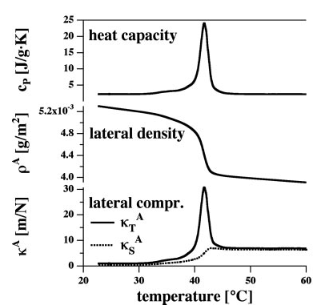
\includegraphics[width=0.5\textwidth]{HJ Fig 2.png}
    \caption{Data from Heimburg and Jackson describing the heat capacity of DPPC large unilamellar vesicle (Top), lateral area density, $\rho^A$ (Middle), and the corresponding lateral compressibility (Bottom) (isothermal area compressibility, solid curve, corresponding to a low-frequency case and adiabatic area compressibility, dotted line, corresponding to a 5-MHz ultrasonic experiment), as calculated from the heat capacity.}
    \label{fig:HJF2}
\end{figure}
The following equations can then be derived 
\begin{equation}
\begin{split}
    \kappa^V_T = \kappa^V_{T,0} + \Delta \kappa^V_T = \kappa^V_{T,0} + \frac{\gamma_V^2T}{\langle V\rangle} \Delta c_P \\
    \kappa_T^A = \kappa^A_{T,0} + \Delta \kappa^A_T = \kappa^V_{T,0} + \frac{\gamma_A^2T}{\langle A\rangle} \Delta c_P \\
\end{split}
\end{equation}
As seen in Figure \ref{fig:HJF2}, both elastic constants and the heat capacity change drastically around the miscibility temperature. There is also a significant drop in density around this temperature. This effectively acts as a spring that softens as it gets compressed. This is important as the propagation speed $c_0$ is proportional to $1/\sqrt{\rho \kappa_S}$ where $\kappa_S$ is the isentropic compressibility. This nonlinearity is what allows for the propagation of solitons. Using Maxwell's Relations, we can show that 
\begin{equation}
\begin{split}
    \kappa_S^V = \kappa_T^V - \frac{T}{\langle V \rangle c_P}\left( \od{V}{T} \right)^2_P \\
    \kappa_S^A = \kappa_T^A - \frac{T}{\langle A \rangle c_P}\left( \od{A}{T} \right)^2_P
\end{split}
\end{equation}
Without any dispersion effects, we consider the acoustic wave equation we derived at the beginning of this section but with nonuniform density and compressibility,
\begin{equation}
     \pdt{}{t} \Delta \rho^A = \pd{}{x}\left( \frac{1}{\kappa^A_S\rho^A} \left(\pd{}{x}\Delta \rho^A\right)\right)   
\end{equation}
where $\Delta \rho^A = \rho^A - \rho_0^A$ is a function of $x$ and $t$. Around miscibility temperature, the lateral compressibility is not constant and therefore let us Taylor expand the propagation speed it to the second order term
\begin{equation}
    c^2 = \frac{1}{\rho^A \kappa^A_S} = c_0^2+p\Delta\rho^A + q(\Delta\rho^A)^2+...
\end{equation}
They then proceed to empirically add a dispersive term $-h\pdfo{\Delta \rho^A}{x}$ for $h>0$. Our equation now becomes 
\begin{equation}
        \pdt{}{t}\Delta \rho^A = \pd{}{x}\left[ (c_0^2+p\Delta \rho^A +q (\Delta \rho^A)^2)\pd{}{x}\Delta \rho^A\right] - h \pdfo{}{x}\Delta \rho^A
\end{equation}
We shall now find the dispersion relation for low amplitude solutions by using the ansatz $\Delta \rho^A = u=\rho_0^A \sin (\omega t-kx)$. Since we are concerned with low amplitude solutions, anytime $u$ is multiplied with itself or its derivatives, they annihilate each other.
\begin{equation}
\begin{split}
    -\omega^2u = \pd{}{x}(-c_0^2u')-hk^4u =-c_0^2k^2u-hk^4u\\
    \Rightarrow \omega^2 = c_0^2k^2+hk^4\\
    \Rightarrow c_p^2 = v^2 = \frac{\omega^2}{k^2}=c_0^2+hk^2
\end{split}
\end{equation}
Since $h$ is very small, we shall first ignore it to obtain the relation $k^2= \omega^2/c_0^2$. We can then plug it back into the relation we obtained above to achieve an approximation such that the phase velocity $c_p$ (not to be confused with the heat capacity $c_P$) is a function of the angular frequency and not the wave number.
\begin{equation}
    v^2 \approx c_0^2 + h\frac{\omega^2}{c_0^2}
\end{equation}
We now solve the acoustic wave equation with fourth-order dispersion by performing a change of variables for traveling wave solutions $z=x-vt$.
\begin{equation}
    v^2\pdt{}{z}\Delta \rho^A = \pd{}{z} \left[ (c_0^2 +p\Delta \rho^A + q(\Delta \rho^A)^2) \pd{}{z} \Delta \rho^A\right] - h \pdfo{}{z}\Delta \rho^A
\end{equation}
We shall also impose localizing boundary conditions such that $u=\Delta \rho^A \rightarrow 0$ as $|z| \rightarrow \infty$. Integrating both sides once and rearranging, we get the equation 
\begin{equation}
    h\frac{\partial^3 u}{\partial z^3}  = (c_0^2-v^2)\pd{u}{z} + pu \pd{u}{z}+qu^2\pd{u}{z}
\end{equation}
We can integrate this once more by recognizing the chain rule.
\begin{equation}
    h \pdt{u}{z} = (c_0^2-v^2)u + \frac{1}{2} pu^2+\frac{1}{3} qu^3 \label{eq:5.19}
\end{equation}
From this point we can determine that in order for the solutions to be localized, we must have that $v< c_0$. For large $|z|$, due to the localization conditions, $\Delta \rho^A $ is very small and so we can ignore higher powers of it. This leaves us with the second order equation 
\begin{equation*}
    h\pdt{u}{z} = (c_0^2-v^2)u \rightarrow u \sim e^{-|z|\sqrt{\frac{1}{h}(c_0^2-v^2)}}
\end{equation*}
and so thus, $v<c_0$ or else we have oscillatory solutions. Multiplying both sides of \eqref{eq:5.19} by $\pd{u}{z}$, we can apply the reverse chain rule logic again to get 
\begin{equation}
    \frac{h}{2} \left(\pd{u}{z} \right)^2 = \frac{1}{2}(c_0^2-v^2)u^2+\frac{1}{6}pu^3 + \frac{1}{12}qu^4 \label{eq:5.20}
\end{equation}
Since the left hand side is positive definite and we have a compression pulse, there must be a maximum (and at that point, the $\pd{u}{z} = 0$). It is also symmetric about this maximum since if you take the square root of both sides, you end up with the first characteristic derivative equaling a plus minus and so hence, the rate of change in the density is the same but with opposite parities. As we have determined above, $v<c_0$ and so thus $(c_0^2-v^2) >0$ and the same can be said about $q$. The reasoning for this is because near the transition temperature, the lipids become extremely compressible and speed drops to a minimum. After this point, the lipids pack close together and become stiff and so the propagation speed increases. If $q<0$, then the propagation speed would drop to negative infinity which is unphysical. Therefore to keep things physical and to obey the second derivative test for the propagation speed as a function of $\Delta \rho^A$, $q$ must be positive. Therefore to force real roots, $p$ must be negative. At the maximum, where the left hand side is 0, and for $v \approx c_0$ (but of course still less than $c_0$), the soliton amplitude is small and so thus we can ignore the fourth order term. This allows us to approximate the soliton amplitude to be 
\begin{equation}
\begin{split}
    0=(c_0^2-v^2)+\frac{p}{3}u \rightarrow -\frac{p}{3}u=(c_0^2-v^2) \\
    \Rightarrow\Delta\rho^A=u=\frac{3(c_0^2-v^2)}{|p|}
\end{split}    
\end{equation}
This effectively means that the solitons vanish as $v\rightarrow c_0$, but on the other hand, they will not form if the soliton is too slow. We can observe this happening when the right hand side of \eqref{eq:5.20} has only one solution (as with two solutions, it is a real valued soliton and with no solutions, the soliton doesn't exist) when $\pd{u}{z}=0$. We then take the determinant and set it equal to zero to get
\begin{equation}
\begin{split}
    \frac{1}{9}p^2-\frac{2}{3}q(c_0^2-v_{\text{limit}}^2) &=0 \\
    \Rightarrow c_0^2-v_{\text{limit}}^2 &=\frac{p^2}{6q} \\
    \Rightarrow v^2_{\text{limit}} &= c_0^2-\frac{p^2}{6q}
\end{split}
\end{equation}
We can figure out the amplitude at this critical point by using the vertex of the parabola $\Delta \rho^A_{\text{max, limit}} = -\frac{b}{2a}$ for the quadratic equation $ax^2+bx+c=0$.
\begin{equation}
    \Delta \rho^A_{\text{max, limit}} = -\frac{p/3}{2(q/6)} = \frac{|p|}{q}
\end{equation}
Using Chapman-Gouy theory for electric double layers, the energy density for the soliton is 
\begin{equation}
    e_{\text{sol}} = \frac{c_0^2}{\rho_0^A}(\Delta \rho^A)^2 + \frac{p}{3\rho_0^A}(\Delta \rho^A)^3 + \frac{q}{6\rho_0^A}(\Delta \rho^A)^4
\end{equation}
and one can extract the total energy of soliton by integrating over the entire profile. This energy density also includes the contributions from the electrostatic potential which is a consequence of the compression of the membrane when there is a charge asymmetry across it. The voltage is linear proportional to $\Delta \rho^A$ and we normalize it to the maximum potential $V_0$ when $\Delta \rho^A = \Delta \rho^A_{\text{max, limit}}$ using the relation 
\begin{equation*}
    V = V_0\left( \frac{\Delta \rho^A}{\Delta \rho^A_{\text{max, limit}}} \right)
\end{equation*}
and therefore substituting this into the energy density of a capacitor, we get that 
\begin{equation}
    e_{\text{cap}} =\frac{1}{2}c_m\left(\frac{V_0\Delta \rho^A}{\Delta \rho^A_{\text{max, limit}}} \right)^2
\end{equation}

\newpage



\section{Das and Schwarz}
\textbf{Solitons in Cell Membranes}\\
Their main claim in this paper is that they are analyzing the the cell membrane as a smectic C* (SmC*) liquid crystal model. Smectic refers to the phase of the liquid crystals which is when they form parallel layers (which in this case, is the lipid bilayer). The C refers to their director tilt. The director is the direction in the which the longitudinal axis of the liquid crystal points. In Smectic A liquid crystals, the director points in the normal direction to the smectic planes but in Smectic C crystals, the director is offset from the normal by a certain angle. The * refers to the fact that the liquid crystals are chiral. This allows for the model to include electric polarization, anisotropic, and liquid properties of the lipid molecules. According to Das and Schwarz, they claim that the SmC* model has an added innate, transverse ferroelectric property that allows for an electric field to exist within the plane of the lipids along with the longitudinal transmembrane field. They then obtain a Landau-de Gennes like free energy model that contains elastic, fluctuation, polarization, and ferroelectric terms that allow for solitons to propagate. More specifically, minimizing this free energy model and equating it to a damping terms allows them to recover Fitzhugh-Nagumo like PDEs (which simplify the Hodgkin-Huxley model from a 4D phase space to one with just two variables). \\\\
\begin{figure}[htbp]
    \centering
    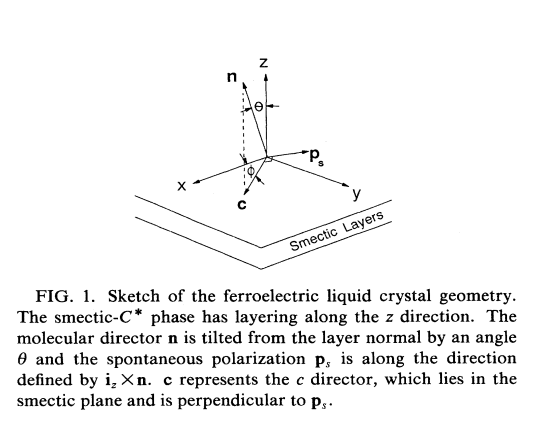
\includegraphics[width=0.5\linewidth]{Das Schwarz Fig 1.png}
    \caption{Figure 1 from Das and Schwarz \textit{Solitons in Cell Membranes.}}
    \label{fig:DSFO}
\end{figure}\\
It is the chirality of the lipid molecules that allow for the individual dipole moments to constructively add and lead to an overall polarization vector $\vb{p}_s$ that has components within the smectic plane and along the normal. The free energy of this phase is noted in \textit{Solitons in Liquid Crystals} by L. Lam to be 
\begin{equation}
    F=\bigintsss dx\left[ \frac{K\theta ^2}{2}\left( \od{\phi}{x}+q_0\right)^2 - \frac{\varepsilon_a \theta^2}{8\pi}E^2\sin^2\phi - p_s\theta E\cos \phi \right] \label{eq:6.1}
\end{equation}
where we have adopted the frustrating physicist convention of putting the integrand after the differential. We have $\phi$ to be the azimuthal angle (as seen in Figure \ref{fig:DSFO}) and so $\od{\phi}{x}$ is effectively how the change in the lean in space. $q_0$ is the wavevector of the helix and is defined to be $q_0 = \frac{2\pi}{T}$ where $T$ is the natural pitch of the helix. It effectively is the angular frequency around the longitudinal axis of the liquid crystal. In effect, the first term acts as an elastic term that penalizes deviations from the natural pitch of the liquid crystals. The second term acts as the dielectric coupling term and measures how in line the director's projection in the smectic plane, the $\vb{c}$ vector, is with the E-field (which is in the (0,1,0) direction). Due to the anisotropy of the system, they have used the anisotropic dielectric which is axis dependent. Therefore, there is an energy reward for the $c$-director to be in line with the electric field as then, the dipole will be along ``long" axis of the crystal and will be at its strongest. And there is an additional reward for the director's tilt to be within the plane since to have the longitudinal axis completely parallel with the E-field would be the most energetically favorable. The last term is simply the potential energy of a dipole in an external electric field. Again, the chirality of the liquid crystal creates a permanent electric dipole $\vb{p}_s$ and so the potential of a dipole in a electric field is $U = -\vb{p}_s \cdot\vb{E}$.\\\\
We will now use the Euler-Lagrange Equations,
\begin{equation}
    \od{}{t}\left(\pd{L}{q_i} \right) - \pd{L}{\dot{q}_i} = 0
\end{equation}
where the Lagrangian is $L=K-U$, $q_i$ is a state variable in the configuration space $X$ that describes the $i^{th}$ particle of the system, and the dot indicates a derivative with respect to time. As a result of minimizing \eqref{eq:6.1} using the Euler-Lagrange Equations and setting it equal to a damping term, we get 
\begin{equation}
    K\theta^2 \pdt{\phi}{x} + \frac{\varepsilon_a \theta^2}{4\pi}E^2\cos \phi \sin \phi - \theta p_s \sin \phi = \gamma \theta^2 \pd{\phi}{t} \label{eq:6.3}
\end{equation}
While this looks like a forced heat equation, it is actually an overdamped version of the Sine-Gordon Equation. The damped Sine Gordon Equation takes the form 
\begin{equation}
    I\pdt{\phi}{t} + \gamma \theta^2 \pd{\phi}{t} =K\theta^2 \pdt{\phi}{x} + \alpha\sin\phi
\end{equation}
where $I$ is the moment of inertia and $\alpha$ is some constant. The first order time derivative acts as the viscous damping term and in our case, dominates the inertial term and we drop it out of the equation. The Sine-Gordon Equation has been extensively studied and shown to permit soliton solutions. The heat equation being inside \eqref{eq:6.3} does point to the existence of dispersion which is balanced out by the nonlinearity of the sines and cosines. \\\\
Cell membranes are extremely thin (roughly 50-100\AA) and so are practically speaking 2D. This means that they are easily affected by long wavelength thermal fluctuations with the implication that the displacement of membrane $u(x,y,z,t)$ has the conditions $\langle u(x,y,z) \rangle = 0$ and $|u(x,y,z)| \ll 1$. Since we have assumed for practical reasons that the membrane is thin with slow moving ripples, there is no meaningful change in the displacement along the $z$ direction (so $\pd{u}{z} = 0)$ and we write out the layer normal to be 
\begin{equation}
    \vb{n} = \left\langle -\pd{u}{x}, -\pd{u}{y}, 1-\tfrac{1}{2}|\nabla u|^2\right\rangle\label{eq:6.5}
\end{equation}
where $\nabla u$ refers to the 2D gradient (as we have established the change in $u$ with respect to $z$ is 0). In the absnece of the electric field, the free energy of the cell membrane can be expressed as 
\begin{equation}
    F= \bigintsss dV \left[ \frac{1}{2}K_{11} |\lap u|^2 + \frac{\sigma}{d} |\nabla u|^2 \right] \label{eq:6.6}
\end{equation}
We can interpret the first term as the energy cost of splaying where $K_{11}$ is the splay constant. Conventionally, splaying in liquid crystal is conventionally represented by $(\dive{n})^2$. Intuitively, one can imagine splaying as having a fluffy carpet with all of the projections being initially vertical (and hence the directors are normal to the plane). As you step on the carpet, the hairs spread out and you can express this as the divergence of the director field. All of the different types of liquid crystal deformation can be seen in Figure \ref{fig:LCDeform}.
\begin{figure}[htbp]
    \centering
    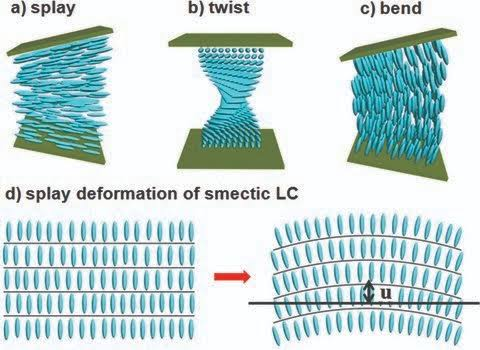
\includegraphics[width=0.5\linewidth]{LC deformations.jpg}
    \caption{The three different types of deformations in liquid crystals. Notice the difference in the director axis between bending and splaying.}
    \label{fig:LCDeform}
\end{figure}
We can show that this conventional way of expressing the splay is the same as the first term in \eqref{eq:6.6}. Let us first take \eqref{eq:6.5} and ignore the second order term in the $z$-component. Now let us take the divergence of it to get 
\begin{equation*}
    \dive {n} = -\pd{}{x}\pd{u}{x} -\pd{}{y}\pd{u}{y} + \pd{}{z}(1))
\end{equation*}
and we can see trivially by squaring that this is equal to $|\lap u|^2$. The second term in \eqref{eq:6.6} represents the required energy to increase the area of the membrane where $\sigma$ is the interfacial surface energy and $d$ is the membrane's thickness. The square of the gradient is fractional increase in the surface area which we can see by parameterizing the membrane via
\begin{equation}
    \vb{r} =\langle x,y,u(x,y) \rangle
\end{equation}
We can now extract scaling factor by finding two tangent vectors to our membrane and finding the magnitude of their cross product. 
\begin{equation}
    \pd{\vb{r}}{x} = \left\langle 1,0\pd{u}{x} \right \rangle \twen \pd{\vb{r}}{y} = \left \langle 0,1,\pd{u}{y} \right \rangle \twen |\,\partial_x \vb{r} \,\times \,\partial_y \vb{r}\,|  = \sqrt{1+|\nabla u|^2}
\end{equation}
Taking the first two terms of the binomial expansion for $\sqrt{1+x}$, we get that the scaling factor is roughly $1+\tfrac{1}{2}|\nabla u|^2$ and so thus to find the fractional increase, we subtract off $dA$
\begin{equation}
    \frac{\Delta A}{A} \approx \left( 1+\tfrac{1}{2}|\nabla u|^2\right) dA - 1dA = \tfrac{1}{2} |\nabla u|^2 dA
\end{equation}
and so $\frac{\Delta A}{A} \sim \tfrac{1}{2} |\nabla u|^2$. Let us now consider an axisymmetric membrane with the change of coordinates $(r,\alpha,x)$ as seen in Figure \ref{fig:DSFT}.
\begin{figure}[htbp]
    \centering
    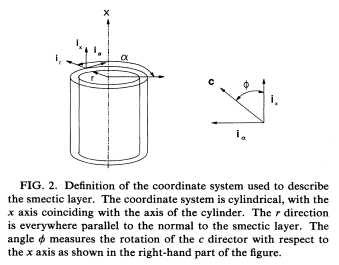
\includegraphics[width=0.5\linewidth]{Das Schwarz Fig 2.png}
    \caption{Figure 2 from Das and Schwarz \textit{Solitons in Cell Membranes}.}
    \label{fig:DSFT}
\end{figure}
Considering that the cylinder is axisymmetric and the membrane is thin,  we have $\pd{u}{\alpha} = \pd{u}{r} = 0$. Performing the $dr$ and $d\alpha$ integrations leaves us with the free energy to be 
\begin{equation}
    F=\pi (R_o^2-R_i^2) \bigintsss dx \left[ \frac{K_{11}}{2} \left( \pdt{u}{x} \right)^2 + \frac{\sigma}{d} \left( \pd{u}{x} \right)^2 \right]
\end{equation}
\begin{figure}[htbp]
    \centering
    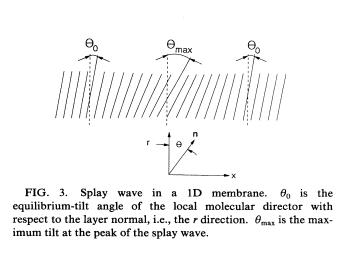
\includegraphics[width=0.5\linewidth]{Das Schwarz Fig 3.png}
    \caption{Figure 3 from Das and Schwarz \textit{Solitons in Cell Membranes.}}
    \label{fig:DSFTh}
\end{figure}
Using Figure \ref{fig:DSFTh}, we have that 
\begin{equation}
    n_x = -\pd{u}{x} = \sin (\theta(x,t)) \twen n_\alpha = 0 \twen n_r = \cos (\theta(x,t))
\end{equation}
We now apply the small angle approximations 
\begin{equation*}
    \sin \theta \approx \theta  \twen \cos \theta \approx 1-\frac{\theta^2}{2!} +\frac{\theta^4}{4!}
\end{equation*}
and the constant manipulations 
\begin{equation*}
    K_b \equiv K_{11}d \twen R_o^2 -R_i^2 = (R_o+R_i)(R_o-R_i) = 2\frac{1}{2}(R_o+R_i)(R_o-R_i) = 2Rd
\end{equation*}
where $R$ is the mean radius, to get 
\begin{equation}
    F= \pi RK_b \bigintsss dx\left[ \left( \pd{\theta}{x}\right)^2+ \frac{4\sigma}{K_b}\left( \theta^2 - \frac{\theta^4}{3}\right) \right]
\end{equation}
Their is good alignment between the experimental and calculated values for the bending constant but this only works for SmA crystals. For SmC crystals, we must start from the SmC free energy density
\begin{equation}
    F' = \frac{1}{2}K^0 \Bigg|\pd{\bs{\xi}}{z} \Bigg|^2 + \frac{1}{2}K^1(\dive{\bs{\xi}})^2 + \frac{1}{2}K^2|\curl{\bs{\xi}}|^2+K^3\left(\bs{\xi} \times \pd{\bs{\xi}}{z} \right) \cdot \left(\curl{\bs{\xi}}\right)
\end{equation}
where $\bs{\xi}$ is the order parameter given by $\bs{\xi} = (\xi_1,\xi_2)$ where $\xi_1 =n_xn_z= \sin \theta \cos \theta \cos\phi$ and $\xi_2 = n_yn_z = \sin \theta \cos \theta \sin \phi$. This effectively the projection of the director onto the smectic plane (or the $\vb{c}$-director) multiplied by the $z$-component. Assuming $\theta$ is very small and ignoring any $z$ dependence on $\theta$ or $\phi$ along with adopting the one constant approximation ($K^0=K^1=K^2=K^3$ which does have experimental backing), we get 
\begin{equation}
    F' = \frac{1}{2}K\left[ (\nabla \theta)^2+\theta^2(\nabla \phi)^2\right] + 4\sigma \left( \theta^2 -\frac{\theta^4}{3}\right)
\end{equation}
The first two terms are the fluctuation terms and the third is an elastic. Since the smectic layer is in the form of a cylinder, we require higher order elastic terms. The next steps are omitted due to how messy they are but generally Das and Schwarz are attempting to write a thin-layer elastic energy model by Taylor expanding around small $\theta$, excluding odd powers (since we require $\theta$ and $-\theta$ to exhibit the same energetic cost), and minimizing with respect to $\phi$. After splitting it into a bunch of cases, the most likely case leads to the model 
\begin{equation}
\begin{split}
    w_{\text{layer}} &\approx \frac{K_{11}}{2R^2} + \frac{1}{2R^2}[A\theta^2+B\theta^4 + O(\theta^6)] \\
    A &\equiv \frac{(\overline{A}_{12} + \overline{A}_{11})(\overline{A}_{21} + \overline{A}_{11})}{(\overline{A}_{12} + \overline{A}_{21} + 2\overline{A}_{11})} \\
    B &\equiv \frac{\left\{(\overline{A}_{12} + \overline{A}_{11})(B_{21} + B_{11}) + (\overline{A}_{21} + \overline{A}_{11})(B_{12} + B_{11}) - \frac{(B_{12} + B_{21} + 2B_{11})(\overline{A}_{12} + \overline{A}_{11})(\overline{A}_{21} + \overline{A}_{11})}{(\overline{A}_{12} + \overline{A}_{21} + 2\overline{A}_{11})}\right\}}{(\overline{A}_{12} + \overline{A}_{21} + 2\overline{A}_{11})}
\end{split}
\end{equation}
Due to both the head groups and hydrocarbon chains being anisotropic, they can be described by the de Gennes stretching vector $\vb{J} = \vb{J}_0 \rho(\vb{J})$. $\vb{J}_0 = \vb{J}_h + \vb{J}_p$ are the average orientations of the hydrocarbon chains and head groups respectively and their norms are the average lengths of these molecules. $\rho(\vb{J})$ is the lateral density given the stretching vector $\vb{J}$. We can therefore define a polarization vector $\vb{p} = \langle \vb{X}\rangle \vb{J}$ where $\langle \vb{X} \rangle$ is a tensor averaged over the motion of the lipid molecules. There is a component parallel to the plane $\vb{p}_s$ and one parallel to the layer normal $\vb{p}_r$. For a curved bilayer (such as the cross section of a cylindrical axon), the longitudinal component of the polarization vector has a magnitude of 
\begin{equation}
    p_r = e\left( \frac{1}{R_1}+\frac{1}{R_2} \right)
\end{equation}
where $e$ is the flexoelectric coefficient and $R_1$ and $R_2$ are the principal radii of curvature. The flexoelectric coefficient can be calculated using the formula
\begin{equation}
    e= - \left( \od{\mu}{A} \right)_{\bar{A}}
\end{equation}
where $\mu$ is the normal component of the lipid dipole moment and $\bar{A}$ is the area per head group of a nonstretched lipid bilayer. The transverse polarization vector, which is within the plane (and so therefore in a cylindrical symmetry, would be pointing tangential to the surface), can be represented using the expression 
\begin{equation}
    \vb{p}_s - \mu_p(\vb{n} \cdot \vb{i}_z)(\vb{i}_z \times \vb{n})
\end{equation}
where $\vb{i}_z$ is once again the layer normal. One can see that if the lipids are straight up (and so $\vb{n} \parallel \vb{i}_z$), the cross product will equal zero and so there is no transverse polarization which makes sense. The constant $\mu_p$ just combines a bunch of different things together such as the dipole moment or anisotropic polarizability and so shall thus be omitted. For a multicomponent mixture with different chiral lipid molecules, this constant is 
\begin{equation}
    \mu_p = \sum x_j x_k\mu_{jk}
\end{equation}
where $x_j$ is the mole fraction of the $j^{th}$ species and $\mu_{jk}$ is determined by the interaction between a molecule of species $j$ and species $k$. However, not all lipids are chiral and so now let us consider a mixture with chiral lipid A and achiral lipid B. The constant is now given by 
\begin{equation}
    \mu_p = \mu_{AA}x^2_A+\mu_{AB}x_Ax_B
\end{equation}
and $\mu_{BB}$ is zero since although there still may be some interactions between two achiral molecules, statistically there are equal quantities of each direction their dipoles may point and therefore should cancel out. Collecting everything together and introducing some other variables and functions (which will be omitted for brevity's sake), we arrive at the final free energy model.
\begin{equation}
\begin{split}
    F = \int dx \left\{ \pi R K_b \left[ \frac{d\theta}{dx} \right]^2 + \pi R K_b \left[ \frac{1}{R} - C_0 \right]^2 + \left[ \left[ \frac{\pi A d}{R} + 4\sigma\pi R \right] - \pi R d \Xi(\xi) \mu_p^2 \cos^2\xi \right] \theta^2 \right. \\ \left.+ \left[ \frac{\pi B d}{R} - \frac{4\sigma\pi R}{3} \right] \theta^4  - 2\pi R d \Xi(\xi) \mu_p E \theta \sin\xi \cos\xi - \pi R d E^2 \sin^2(\xi) \Xi(\xi) \right\}  \label{eq:6.21}
\end{split}
\end{equation}
The most important thing to notice is the coupling between $E$ and $\theta$ in the second to last term. This directly ties the propagation of electric fields with mechanical deformations within the liquid crystal bilayers. It implies that one can stimulate the propagation of electric fields by a mechanical perturbation (which matches the observations cited by Heimburg and Jackson when rejecting the Hodgkin-Huxley model) and vice versa. It is also worth noting that solitons cannot exist when the molecules are achrial as the field coupling term would be zero unless there is some other mechanism connecting the two that is not present in this model. \\\\
\textbf{Fitzhugh-Nagumo Equations}\\
The first part of this section will give a brief introduction to the Van der Pol Oscillator before we transition into a brief overview of the Fitzhugh paper before we return to the Das and Schwarz paper. The Nagumo paper has been skipped because the analysis that is interesting to me has been replicated by Das and Schwarz. \\\\
The Van der Pol oscillator is a non-conservative oscillator with nonlinear damping that obeys the equation 
\begin{equation}
    \odt{x}{t} = \mu(1-x^2) \od{x}{t} -x
\end{equation}
where $x$ is usually the coordinate and $\mu$ is a constant indicating the strength of the damping. By Li\'{e}nard's Theorem, the system has a unique and stable limit cycle which is what Van der Pol originally discovered when working with vacuum tubes. Under the Li\'{e}nard transformation $y=x-\tfrac{1}{3}x^3 - \tfrac{1}{\mu}\dot{x}$, we can rewrite the equation as 
\begin{equation}
\begin{split}
    \dot{x} &= \mu(x-\frac{1}{3}x^3-y) \\
    \dot{y} &= \frac{1}{\mu}x
\end{split}
\end{equation}
The other commonly used transformation is $\dot{x} = y$ which leads to the equations 
\begin{equation}
\begin{split}
    \dot{x}& = y\\
    \dot{y} &= \mu(1-x^2)y-x
\end{split}
\end{equation}
In Fitzhugh's original paper, he modeled the neuron as a Van der Pol Oscillator; however, he noted it was not meant to be an accurate model but rather as an example of describing the different physiological states of action potential via a dynamical system like the VdP oscillator. Fitzhugh creates a Bonhoeffer-Van der Pol model using the equations 
\begin{equation}
\begin{split}
    \dot{x} &= c(y+x-\tfrac{1}{3}x^3+z) \\ 
    \dot{y} &= -\tfrac{1}{c} (x-a+by)
\end{split}
\end{equation}
where we have the conditions
\begin{equation}
    1-\frac{2b}{3} < a < 1 \twen 0 < b<1 \twen b<c^2
\end{equation}
Both $a$ and $b$ are constants and $z$ corresponds with the stimulus intensity which is somewhat analogous to the current in the Hodgkin-Huxley model. There are two nullclines: one linear that corresponds with $\dot{y}=0$ and one N-shaped cubic that corresponds with $\dot{x} = 0$. They meet at a fixed/stable point $P(x_1,y_1)$. Taylor expanding around this fixed point and making the change of variables $\xi=x-x_1$ and $\eta = y-y_1$ we get
\begin{equation}
\begin{split}
    \dot{\xi} &= c(\eta + (1-x_1)^2\xi +x_1\xi^2+\tfrac{1}{3}\eta^3) \\
    \dot{\eta} &= - \tfrac{1}{c}(\xi +b\eta) 
\end{split}
\end{equation}
By only considering the linear terms and omitting those of higher order, we can then take the matrix of coefficients to be 
\begin{equation}
    M= \begin{bmatrix}
        (1-x_1^2)c &c \\
        -\frac{1}{c} & -\frac{b}{c}
    \end{bmatrix}
\end{equation}
According to one of Lyapunov's theorems, this has the same stability as the original set of differential equations. Intuitively, we are just zooming in very close on the fixed point to the point where only the linear contributions matter. Finding the eigenvalues of matrix, we get the determinant
\begin{equation}
    \det(M-\lambda I) = \lambda^2 + \left[ \frac{b}{c} - (1-x_1^2)c \right]\lambda + [1-(1-x_1)^2b] = 0
\end{equation}
The following three statements are equivalent 
\begin{enumerate}
    \item The point $(x_1,y_1)$ is stable
    \item The real parts of the eigenvalues of M are less than 0
    \item $\frac{b}{c}-(1-x_1^2)c>0$ and $1-(1-x_1^2)b>0$
\end{enumerate}
We can effectively cheat around actually finding the eigenvalues by nothing that the roots to the polynomial equation $\lambda^2+B\lambda +C=0$ have negative eigenvalues if $B>0$ and $C>0$. As a result, the fixed point is unstable for $|x_1| \leq (1-\frac{b}{c^2})^{\frac{1}{2}}$. The condition $1-x_1^2< \frac{1}{b}$ is always satisfied since $0<b<1$. For large values of $c$, the instability region is effectively from $(-1,1)$. By looking at the nullclines along $y=-x+\tfrac{1}{3}x^3-z$ and $y=\frac{a-x}{b}$, we see that the fixed point $P$ is dependent on $z$ and hence $z$ has its own region of instability. $z$ is an external stimulus so if a certain $z$ leads to an unstable fixed point, the neuron will constantly fire but within stable regions, the neuron rests. If $z$ is negative, the neuron goes through all the states with a wide limit cycle. \\\\
At rest when $n$ and $h$ (from the Hodgkin Huxley model) are frozen, there exists three fixed points. During an action potential, $n$ and $h$ change which leads to a bifurcation such that there is only one remaining fixed point. This forces the neuron back to rest. Fitzhugh noticed that since both $n$ and $h$ behave similarly, he could replace them with their average $w=\tfrac{1}{2}(n-h)$ and that the $nh$ plane could be projected onto this ``w-axis." One can do something similar with the voltage $V$ and $m$ using the transformation $u=V-36m$.\\\\
To find the steady state curve, we travel along the $\dot{x}=0$ nullcline and hold $y=y_1$ at its resting value. This allows us to find 
\begin{equation}
    z=-y_1-x+\frac{1}{3}x^3
\end{equation}
By setting $\dot{y}=0$, we find that $y = \frac{x-a}{b}$ and so we can substitute this to get 
\begin{equation}
    z= \frac{x-a}{b} -x+\frac{1}{3}x^3
\end{equation}
This effectively tells you how much current $z$ is required to hold a cell at certain voltage $x$. We shall now return to the Das and Schwarz paper. Let us state the Nernst-Planck equation
\begin{equation}
    Cd\od{E}{t} = -F\sum_j D_j \od{[j]}{x} - \frac{F^2E}{R'T} \sum_jD_j[j] +\sum_jI^p_j \label{eq:NP}
\end{equation}
where $C$ is the capacitance of the membrane, $j\in \{\text{Na}^+, \text{K}^+, \text{Cl}^-\}$, $D_j$ is the diffusion coefficient of the $j^{th}$ species, $F$ is Faraday's constant, $R'$ is the gas constant, and $T$ is the absolute temperature. The first term is the electric current driven by diffusion due to the concentration gradient across the membrane. The second is the current due to the electric field. The last is the current due to active ion pumps. We shall now replace $[j]$ with $[j]_{av}$ which is given by 
\begin{equation}
    [j]_{\text{av}} = \beta_j \left( \frac{C_iV_i + C_eV_e}{V_i+V_e}\right)
\end{equation}
where $V_i$ and $V_e$ are the intra and extracelullar volumes respectively and $\beta_j$ is the partition coefficient which relates the concentration of an ion in the membrane with its bulk concentration by $[j]_i = \beta_jC_i$ and $[j]_e = \beta_jC_e$.\\\\
Under resting conditions with $E=E_0$, the left hand side of \eqref{eq:NP} is zero (since the E-field isn't changing) and so thus we can express the current due to the pumps as 
\begin{equation}
    I^p_j = \frac{FD_j}{d} \Delta [j]_{\text{rest}} + \frac{F^2E_0}{R'T}D_j [j]_{\text{av}}
\end{equation}
The Smectic C* model works under the assumption that the concentration gradient of the ions is dependent on the tilt angle of the lipids. As such, we can have let $\theta = \theta^0_j$ be the angle at which the ion channel for the $j^{th}$ species is completely open. Taylor expanding around this point, we get 
\begin{equation}
    [j]_e-[j]_i = f(\theta) = f(\theta^0_j) + (\theta - \theta^0_j)f;'(\theta^0_j) +... = (\theta - \theta^0_j)f;'(\theta^0_j)
\end{equation}
This is done by neglecting higher order terms in the expansion and that if the completely open, then the concentration should collapse and so thus 
\begin{equation}
    f'(\theta^0_j) = \frac{\Delta [j]_{\text{rest}}}{\theta^p_j - \theta^0_j}
\end{equation}
Substituting this expression into \eqref{eq:NP} and doing some algebraic manipulations, we get 
\begin{equation}
    \od{E}{t} + \frac{F^2E}{R'TdC}\sum_j D_j[j]_{\text{av}} = \frac{F}{d^2C}\sum_jD_jf'(\theta^0_j) - \frac{F\theta}{d^2C} \sum_jD_jf'(\theta^0_j) + \frac{F}{Cd^2}\sum_j D_j \Delta [j]_{\text{rest}} + \frac{F^2E_0}{R'TCd}\sum_j D_j [j]_{\text{av}} \label{eq:6.37}
\end{equation}
Minimizing \eqref{eq:6.21} with respect to $\theta$ via the Euler-Lagrange equations and equating it to the damping term $\gamma \pd{\theta}{t}$, we get 
\begin{equation}
    \gamma \pd{\theta}{t} = \pi RK_b \pdt{\theta}{x} -(a\theta^3-b\theta -\tilde{c}E) \label{eq:6.38}
\end{equation}
where 
\begin{equation*}
    a \equiv 4pi R\left( \frac{Bd}{R^2} - \frac{4\sigma}{3}\right) \twen b\equiv 2\pi R \left[ -\left( \frac{Ad}{R^2} + 4\sigma\right) + d\Xi(\xi)\mu_p^2\cos^2\xi \right] \twen \tilde{c} \equiv \pi R d\mu_p\Xi(\xi)\sin\xi\cos\xi 
\end{equation*}
By looking at \eqref{eq:6.37} and \eqref{eq:6.38}, we can compare them to the Fitzhugh-Nagumo equations which take the form 
\begin{equation}
\begin{split}
    &h_0 \pdt{u}{x} = \frac{1}{c_0}\pd{u}{\tau} + \left( \frac{u^3}{3}-u-w\right)\\
    &c_0 \pd{w}{\tau} +b_0w = a_0-u
\end{split}
\end{equation}
This can be done using the change of variabels 
\begin{equation}
    \begin{split}
        \tau &\equiv \frac{t}{(\gamma / \beta\bar{c})^{1/2}} \twen u \equiv \left[ \frac{3a}{b} \right]^{1/2} \theta \twen 
b_0 \equiv \frac{bF^2}{\beta\bar{c}R'TdC} \sum_j D_j[j]_{\text{av}}  \\
w &\equiv \frac{\sqrt{3\bar{c}}a^{1/2}}{b^{3/2}}E, \quad h_0 \equiv \frac{\pi R K_b}{b} , \quad c_0 \equiv \frac{b}{\sqrt{\bar{c}\gamma\beta}} , \\
a_0 &\equiv \left[ \frac{3a}{b\beta^2} \right]^{1/2} \Bigg[ \frac{F}{Cd^2} \sum_j f'(\theta_j^0)\theta_j^0 D_j 
 + \frac{F}{Cd^2} \sum_j D_j \Delta[j]_{\text{rest}} 
 + \frac{F^2 E_0}{R'TCd} \sum_j D_j[j]_{\text{av}} \Bigg] \\
 \beta &\equiv \frac{F}{Cd^2}\sum_j D_j f'(\theta^0_j)
    \end{split}
\end{equation}
If we eliminate $E$ by combining both equations, we obtain 
\begin{equation}
    c_0h_0 \frac{\partial^3 u}{\partial \tau \partial x^2} + b_0h_0\pdt{u}{x} = \pdt{u}{\tau}-c_0\left[ \left( 1- \frac{b_0}{c_0^2} \right)-u^2 \right]\pd{u}{\tau} + (1-b_0)u + \frac{b_0}{3}u^3-a_0
\end{equation}
The behavior of the solution approaches a soliton shape when considering the localizing boundary conditions. 



\end{document}
